\documentclass[../thesis.tex]{subfiles}

\begin{document}

\section{Improving lubrication representation\label{sec:eff}}

\subsection{Non-continuum molecular effects}

\subsection{Internal circulation of fluid drops}

\subsection{Numerical method to compute collision efficiency}

The numerical method for computing the collision efficiency is based on the Lagrangian particle tracking. In the modeled system, the relative motion of two unequal aerodynamically interacting droplets settling under gravity in quiescent air is considered. The droplets are treated as non-deformably spherical particles that are either fluid (having an internal Stokesian circulation) or rigid (non-deformable and solid). The larger droplet assumed here is of the radii $a_1=10, 20,$ and 30~$\mu$m, while the radii of the smaller one is defined by the parameter $\lambda= a_2/ a_1$. In each simulation series, $\lambda$ varies in the range $0.05\leq\lambda\leq0.99$. For such a setting the inertia of the surrounding fluid, i.e.\ air, is negligible. To compute the collision efficiency, the far field off-center horizontal separations for the grazing trajectories need to be determined. In other words, it is necessary to find the maximum horizontal shift beyond the area of aerodynamic interaction for which the collision of the droplets may occur. To find this, a modified bisection method was employed. The simulations were initialized with arbitrary values of the shift and successively corrected based on the information whether the droplets collided or not. Each iteration in this procedure is called a generation. Since the collision efficiency is very sensitive to little differences in aerodynamic interaction representations, it is expected that the non-continuum effects or the internal circulation of water inside droplets will have a noticeable impact on the probability of collision. Thus, these effects will be examined by employing force representation models derived based on each effect. Still, the physical properties of surrounding air and water droplets, including the densities $\rho_f = 1.3 \times 10^{-3}$ and $\rho_i=1$~g/cm$^3$, and the dynamic viscosity $\mu_f = 1.7 \times 10^{-4}$~g/(cm~s), remain the same in all simulations. Moreover, two values, $\mu_i = 100\mu_f$ and $\mu_i \to \infty$, are assumed for the dynamic viscosity of water when the internal circulation of droplets is taken into consideration. This model offers a basic understanding of the interaction between a pair of droplets, which can be later employed in a many-body system of interacting droplets.

%\subsubsection{Numerical method}

\begin{figure}%figurefigurefigurefigurefigurefigurefigurefigure
\center
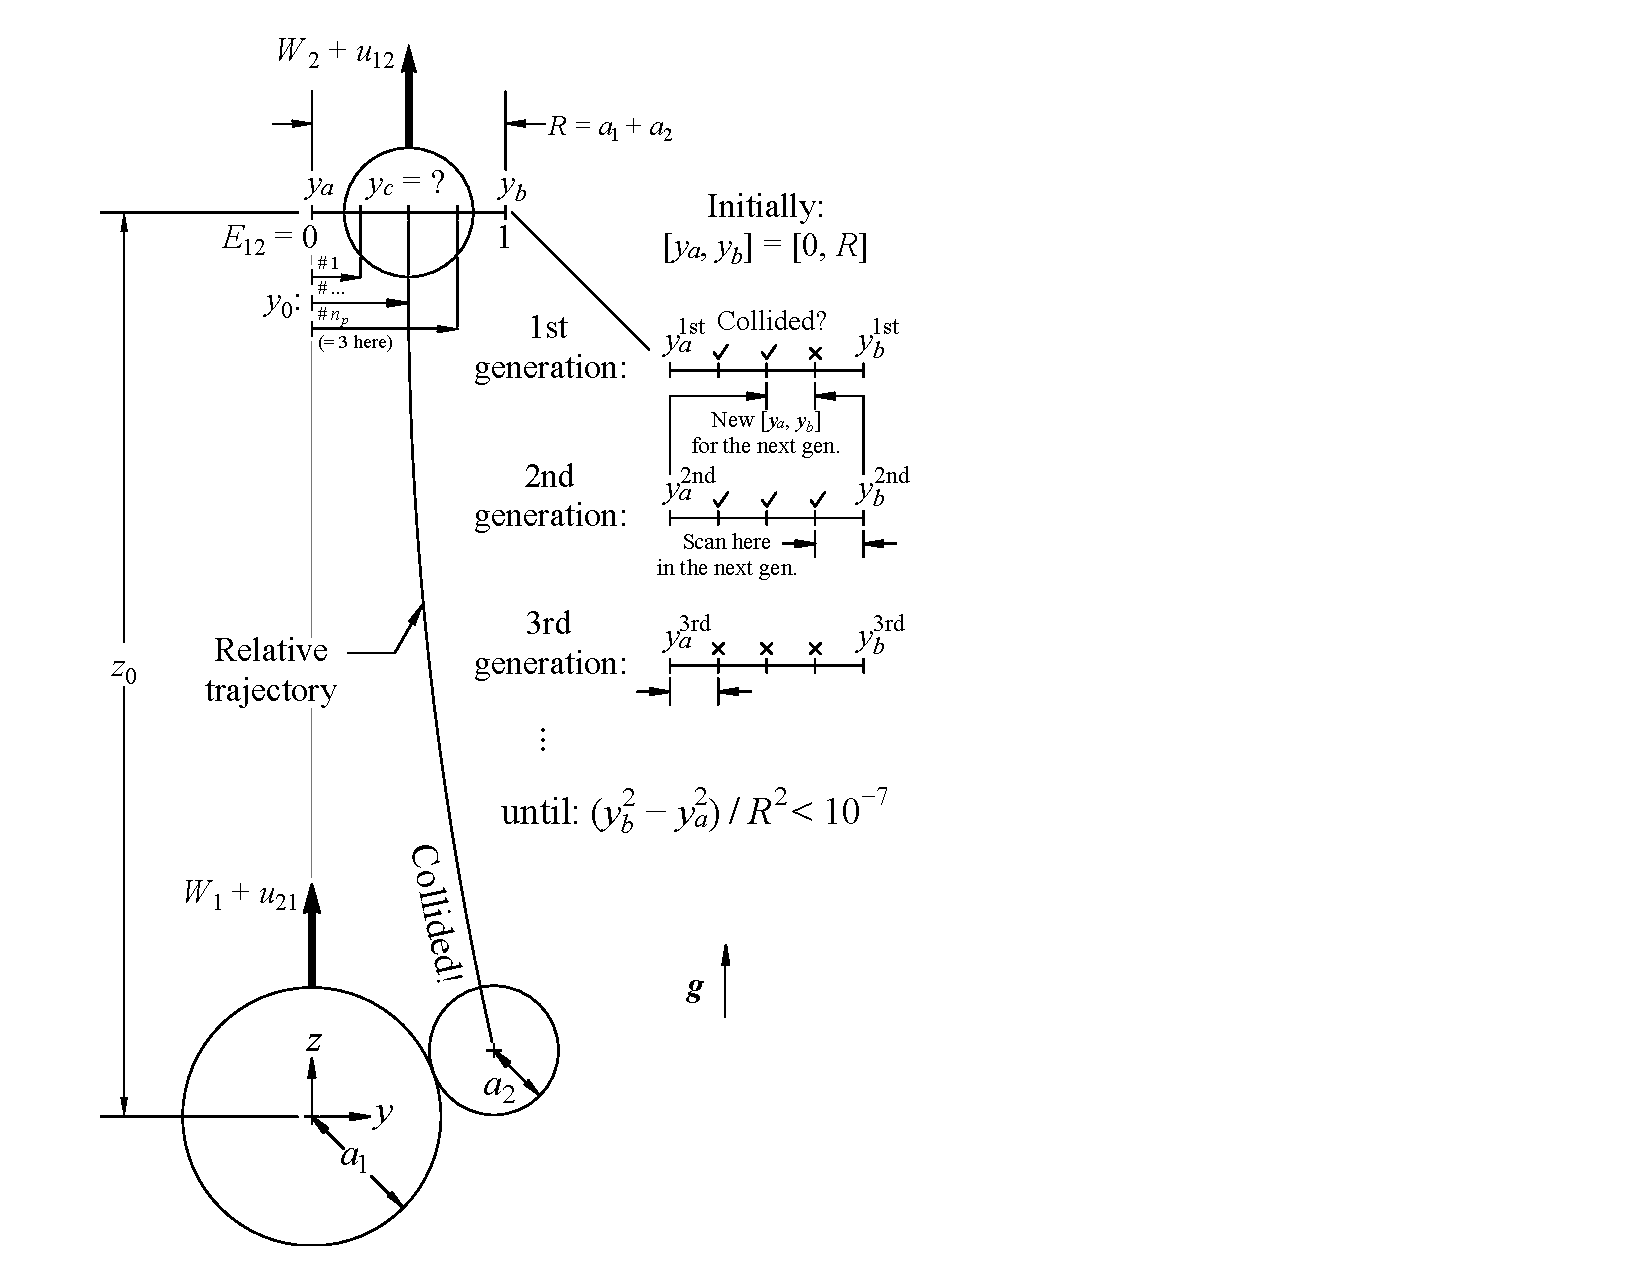
\includegraphics[trim=15mm 05mm 125mm 05mm, clip, width=0.6\textwidth]{../figs/PRF/fig1.pdf}
\caption{A parallel procedure, with $n_\text{c}=3$ here, for evaluation of collision efficiency}
\label{fig:colleff}
\end{figure}

Figure~\ref{fig:colleff} illustrates the methodology to evaluate the collision efficiency. A parallel scanning procedure is used to speed up the convergence rate. Initially, the larger droplet is placed at the origin, \mbox{$\boldsymbol{Y}_1=(0,0,0)$}, and several smaller ones at \mbox{$\boldsymbol{Y}_2=(0,y_0,z_0)$}, each setting being an independent problem. The initial vertical separation is always the same and equal to $z_0 = 50R$, where $R=a_1+a_2$. This distance is large enough to ensure that the collision efficiency does not depend on the initial vertical separation distance. As for the initial horizontal separation distance $y_0(t=0)$, different values are simultaneously considered, \smash{$y_0^{(1)},\dots,y_0^{(n_\text{c})}$}. This configuration comes down to placing $n_\text{c}$ smaller droplets at equally spaced distances within the entire possible (initial) range of collision, namely $[0,R]$. Here $n_\text{c}$ is the number of processes (sub-generations) per generation, each given to a computational (CPU) core. The initial velocities are the terminal velocity of each droplet to which the Stokes disturbance of the other droplet is added to ensure that collision efficiency and droplet trajectories are independent from the initial vertical separation distance, $z_0$. These settings reduce the three-dimensional problem to a quasi-two-dimensional one with the droplets moving only in $y$--$z$ plane and rotating around the axis pointed in $x$ direction. Every sub-generation independently begins to evolve by integrating the equations of motion for each pair of droplets. An entire generation finishes once all of its sub-generations are completed with an outcome, either a collision or not. Based on this information, the range of $y_0$ is narrowed down for the next generation. This procedure continues until the range is narrow enough, where the maximum initial horizontal separation distance leading to a collision, $y_c (\approx y_b \approx y_a)$, is found, providing an estimation for collision efficiency \citep{PK97}:

\begin{equation}
E_{12} = \frac{y_c^2}{R^2}.
\end{equation}
The collision efficiency can alternatively be defined based on the size of larger droplet as $E'_{12} = y_c^2/a_1^2=E_{12}(1+\lambda)^2$, which can be greater than unity \citep{YR96}.

\subsection{Equations of motion}

The acceleration of a pair of inertial particles can be expressed using the following compact notation
\begin{align}
\frac{\text{d} \boldsymbol{V}_i}{\text{d} t} &= \left(1-\frac{\rho_f}{\rho_i}\right)\boldsymbol{g}+\frac{\boldsymbol{F}_i}{m_i}, \qquad i=1,2
\label{eq:acc}
\end{align}
where the first term on the RHS includes gravity and buoyancy. The second term handles all the other forces e.g.\ attractive van der Waals forces, hydrodynamic (aerodynamic, in this case) interaction between the particles (water droplets), etc.

Treating a rigid sphere as a special case, the drag force ($F_i^s$ here $s$ stands for single sphere) exerted by a fluid of viscosity $\mu_f$ on an isolated spherical fluid drop of viscosity $\mu_i$ is (Hadamard--Rybczy{\'n}ski solution in Sec.\ 4.9 of \cite{B00} or Example 4.3 of \cite{KK13}):
\begin{align}
F_i^s = -4\pi\mu_f a_i V_i
\underbrace{\frac{\tfrac{3}{2}\hat{\mu}_r+1}{\hat{\mu}_r+1}}_{\hat{\mu}_d}
=
-4\pi\mu_{fd} a_i V_i,\label{eq:fddrag}
\end{align}
where $\hat{\mu}_r\equiv\tfrac{\mu_i}{\mu_f}$ is the viscosity ratio and $\mu_{fd}\equiv\mu_f\hat{\mu}_d$ is a factor defined for convenience to avoid repetition. Here, hats indicate the values that are dimensionless. The special case of Stokes drag acting on a rigid sphere, $-6\pi\mu_f a_i V_i$, is recovered when $\hat{\mu}_r\to\infty$ \citep{KK13}. Based on Equation~(\ref{eq:fddrag}), the fluid droplet inertial response time is defined as
\begin{align}
\tau_i \equiv \frac{m_i}{4\pi\mu_{fd}a_i},\label{eq:tau}
\end{align}
yielding terminal velocities
\begin{align}
W_i = \left(1-\frac{\rho_f}{\rho_i}\right)\tau_i g.\label{eq:w}
\end{align}
It is worth noting that the inertia ($\tau_i$) of the liquid particle (fluid drop) is larger than that of the rigid particle, and thus its settling velocity is correspondingly faster.

Equation~(\ref{eq:acc}) can be rewritten using the definitions given in Equations~(\ref{eq:tau}) and (\ref{eq:w}). Moreover, the force representing the aerodynamic interaction ($F_i^{AI}$) can be normalized by the Stokes drag factor for a single spherical fluid drop and then expressed in terms of the velocity perturbation, namely, \mbox{$u_i \equiv F_i^{AI} / -4\pi\mu_{fd}a_i$}. Accordingly, the equations of motion for a pair of particles reduce to
\begin{align}
\frac{\text{d} \boldsymbol{V}_i}{\text{d} t} &= \frac{\boldsymbol{W}_i-\boldsymbol{u}_i}{\tau_i}, \label{eq:eqm1} \\
\frac{\text{d} \boldsymbol{Y}_i}{\text{d} t} &= \boldsymbol{V}_i, \label{eq:eqm2} \\
\frac{\text{d} \boldsymbol{\Omega}_i}{\text{d} t} &= \frac{\boldsymbol{T}_i}{I_i}. \qquad \text{(only rigid)} \label{eq:eqm3}
\end{align}
Here, $\boldsymbol{Y}_i$ and $\boldsymbol{V}_i$ denote the position and velocity of the droplets, respectively. Equation~(\ref{eq:eqm3}) applies only to rigid spherical particles with angular velocities, torques, and moments of inertia referred to by $\boldsymbol{\Omega}_i$, $\boldsymbol{T}_i$, and $I_i$, correspondingly. For fluid drops, this equation must be replaced with $\text{d}\boldsymbol{L}/\text{d}t = \boldsymbol{T}$ where the angular momentum is defined as $\boldsymbol{L} = \int_V\boldsymbol{r}\times\boldsymbol{U}\rho\text{d}V$ over the drop volume, with $\boldsymbol{r}$ being the radial vector from the center of the drop and $\boldsymbol{U}$ the surrounding fluid velocity. \cite{Z80} proved that the hydrodynamic torque acting on a fluid drop is always zero. The proof holds even for a Navier--Stokes flow inside each drop:
\begin{subequations}
\begin{align}
\boldsymbol{T} &= \oint_S \boldsymbol{r} \times \boldsymbol{\sigma}_f^{(\boldsymbol{\hat{n}})} \text{d}S \\
&= \int_V\boldsymbol{r}\times\boldsymbol{\nabla \cdot \sigma}_i \text{d}V \label{eq:proofb} \\
&= \int_V\boldsymbol{r} \times \rho \frac{\text{D}\boldsymbol{U}}{\text{D}t} \text{d}V \\
&= \frac{\text{d}\boldsymbol{L}}{\text{d}t}
\end{align}
\end{subequations}
which is zero in the case of Stokes flow, $\boldsymbol{\nabla \cdot \sigma}_i = 0$, where $\boldsymbol{\sigma}$ is the stress tensor and $\boldsymbol{\sigma}^{(\boldsymbol{\hat{n}})}$ is the stress vector on the surface $\text{d}S$. Note that Equation~(\ref{eq:proofb}) switches the integration over the external to the internal surface of the drop owing to tangential stress continuity, and employs Gauss theorem to transform this into a volume integral \citep{Z80}. Since angular momentum is automatically conserved for a fluid drop, there is no need to solve an equation equivalent to Equation~(\ref{eq:eqm3}) even for a massive drop with inertia. Moreover, the hydrodynamic torque vanishes when the internal circulation is approximated as a Stokes flow. This is plausible for small atmospheric drops only due to their large dynamic viscosity ratio. 

\subsection{Force and torque representations}

The terms representing the aerodynamic interaction in Equations~(\ref{eq:eqm1})--(\ref{eq:eqm3}) are evaluated using both approximate and exact solutions of the Stokes equation. The torque does not need to be evaluated if the droplet rotation is neglected. An approximate representation of the aerodynamic force is obtained using (i) the Improved Superposition Method (ISM) of \cite{WAG05}. This method was originally developed for modeling systems comprised of solid spherical particles. To employ the ISM for modeling the collision efficiency of water droplets, it first had to be generalized to the case of liquid particles. This method is based on the exact solution to the Stokes flow induced by a single translating sphere. Exact force representations utilized here are based on analytical solutions to the two-sphere problem. We used two alternative solutions available in the literature, namely (ii) twin multipole expansion method, and (iii) solutions in bispherical coordinates system. Finally, we use an (iv) accurate representation of AI which additionally accounts for the non-continuum lubrication effects.

\subsubsection{Hadamard--Rybczy{\'n}ski solution: approximate representation\label{sec:hr}}
Stokes disturbance field generated by a single non-deformably spherical fluid drop of radius $a$ and dynamic viscosity $\mu_i$ moving at the velocity $\boldsymbol{V}$ in a fluid of viscosity $\mu_f$  is \citep{H11,R11}:
\begin{align}
\boldsymbol{u}_\text{St}(\boldsymbol{r};a,\boldsymbol{V}) = &\left[A_1 \left(\frac{a}{r}\right) - 3B_1 \left(\frac{a}{r}\right)^3 \right] \frac{\boldsymbol{V \cdot r}}{r^2} \boldsymbol{r} \nonumber\\
+ &\left[A_1 \left(\frac{a}{r}\right) + \;\; B_1 \left(\frac{a}{r}\right)^3 \right] \boldsymbol{V},
\label{eq:hr}
\end{align}
in which $r = \|\boldsymbol{r}\|$ is the magnitude of the vector connecting the center of the sphere to any arbitrary point at which the disturbance $\boldsymbol{u}_\text{St}$ is felt; $A_1 = \tfrac{2+3\hat{\mu}_r}{4(1+\hat{\mu}_r)}$ and $B_1 = \tfrac{\hat{\mu}_r}{4(1+\hat{\mu}_r)}$ are derived in hydrodynamics textbooks, e.g.\ Example 4.3 in \cite{KK13}. We note that in the limit $\hat{\mu}_r\to\infty$, Equation~(\ref{eq:hr}) converges to the formula representing the Stokes disturbance field generated by a rigid sphere translating in a viscous fluid (Exercise 2.7 in \cite{KK13}).


The ISM of \cite{WAG05} is generalized for spherical fluid drops by replacing the Stokes disturbance velocity field generated by a rigid sphere with Equation~(\ref{eq:hr}). This yields an approximate representation for the forces acting on a pair of liquid, as well as solid, spheres. Since the ISM is based on the superposition of solutions for single spheres, the forces of aerodynamic interactions are accurate only for large separation distances. Nevertheless, the important advantage of ISM is its ability to be extended for a many-body system of interacting particles \citep{AGW07}. It should also be added that the rotational motion is intrinsically not handled by the ISM.

\subsubsection{Resistance functions: exact representation}

The general resistance problem relates the forces and the torques acting on two spheres $(\boldsymbol{F}_i,\boldsymbol{T}_i)$ to their linear and angular velocities $(\boldsymbol{V}_i,\boldsymbol{\Omega}_i)$. This relation is given \cite[e.g.\ Equation~(1.3) in][]{JO84} as follows
\begin{equation}
{\begin{pmatrix}
\boldsymbol{F}_1 \\
\boldsymbol{F}_2 \\
\boldsymbol{T}_1 \\
\boldsymbol{T}_2 \\
\end{pmatrix}}
=\mu_f
{\begin{bmatrix}
\boldsymbol{A}_{11} & \boldsymbol{A}_{12} & \boldsymbol{\tilde{B}}_{11} & \boldsymbol{\tilde{B}}_{12} \\
\boldsymbol{A}_{21} & \boldsymbol{A}_{22} & \boldsymbol{\tilde{B}}_{21} & \boldsymbol{\tilde{B}}_{22} \\
\boldsymbol{B}_{11} & \boldsymbol{B}_{12} & \boldsymbol{C}_{11} & \boldsymbol{C}_{12} \\
\boldsymbol{B}_{21} & \boldsymbol{B}_{22} & \boldsymbol{C}_{21} & \boldsymbol{C}_{22}
\end{bmatrix}}
{\begin{pmatrix}
\boldsymbol{V}_1 \\
\boldsymbol{V}_2 \\
\boldsymbol{\Omega}_1 \\
\boldsymbol{\Omega}_2
\end{pmatrix}},
\label{eq:res}
\end{equation}
in which $\mu_f$ is the dynamic viscosity of the ambient fluid. The resistance tensors $\boldsymbol{A}_{\alpha\beta}$, $\boldsymbol{\tilde{B}}_{\alpha\beta}$, $\boldsymbol{B}_{\alpha\beta}$, and $\boldsymbol{C}_{\alpha\beta}$ are comprised of the resistance functions $X^{\boldsymbol{A}}_{\alpha\beta}, Y^{\boldsymbol{A}}_{\alpha\beta}, Y^{\boldsymbol{B}}_{\alpha\beta}, X^{\boldsymbol{C}}_{\alpha\beta},$ and $Y^{\boldsymbol{C}}_{\alpha\beta}$. A complete set of these functions for two rigid spheres assuming the no-slip boundary condition has been derived making use of twin multipole expansions \citep{JO84}. Each function takes the form of a high-order series in inverse powers of center-to-center separation. The singularities are removed using asymptotic expressions that are valid for nearly touching spheres. The functions depend on the spheres radius ratio $\lambda=a_2/a_1$ and normalized separation distance $s = r/\frac{1}{2}(a_1+a_2)$. Here, $r$ is the distance between the centers of the particles. The functions $X$ and $Y$ handle motion along the line of centers and normal to that, respectively. The indices $\alpha$ and $\beta$ are integers $\{1,2\}$, introduced to distinguish particles in the pair. These resistance functions provide an exact force--torque representation exerted on a pair of rigid spheres that is only valid in the limit of continuum fluid mechanics. Further on, we will discuss the non-continuum lubrication description that is based on these resistances with a modified $X^{\boldsymbol{A}}_{\alpha\beta}$ function.

\subsubsection{Bispherical solutions: exact representation}%%%%%%%%%

The literature offers a number of solutions, both partial for selected cases and complete, to the Stokes equation for a system of two interacting spheres. A brief survey of the exact solutions developed in bispherical coordinates is carried out in Appendix \ref{sec:bi}. A few of them are employed here to obtain the accurate representation of the aerodynamic interactions. For example, the translational motion along the line joining particle centers is handled by an implicit implementation of \cite{SJ26}. In turn, forces and torques driving the relative motion in the direction normal to the line of centers are obtained from \cite{ONM70}. The complexity of the modeled system can be significantly reduced by mapping particle motion onto a (2D) vertical plane. Due to the geometrical setting, there is neither rotation nor torque around the line of centers.

For modeling the motion of a pair of spherical drops, we use the methodology developed by \cite{HHS73} and \cite{Z80}. These solutions enable us to calculate the interactions of particles in the direction parallel and perpendicular to the line connecting their centers. It is worth mentioning that these representations \citep{HHS73,Z80} have already been used by \cite{Z82} to compute the collision efficiency of non-inertial liquid spheres. The simulations performed here use the same method for a more general case of inertial droplets of unequal size.


\subsubsection{Non-continuum lubrication representation}%%%%%%%%%%%%
The analytical solutions to the Stokes equation for two rigid spheres discussed above were developed assuming that the surrounding fluid is a continuous medium. This assumption is valid as long as the gap between the surfaces of the spheres is significantly larger than the mean free path of the fluid molecules. When the collisions of cloud droplets are considered, the discrete molecular structure of air becomes important, and this effect needs to be adequately taken into account. In particular, consequences of non-continuum interactions are the most pronounced for the squeezing flow, i.e.\ a pair of particles approaching each other. For the other types of motion, e.g.\ shearing flow, these effects are less important or even negligible. This is because the tangential mobilities, even under continuum hydrodynamics, remain finite at contact \citep{DRK21a}. In general, the non-continuum lubrication forces are lower, although the reduction depends on the gap between the spheres. 

Depending on the thickness of the gap relative to the mean free path of air molecules, the flow between the spheres falls in different regimes. \cite{SK96} combined several approaches and computed the pressure distribution in the gap between spheres within a wide range of gap sizes. Then, the non-continuum lubrication forces were derived via integrating the pressure over particle surfaces. \cite{DRK21a} have fitted a smooth function $f^\text{nc}$ to these solutions \citep{SK96}, uniformly covering separation distances under different regimes (see Section 4.1 therein). This non-continuum representation converges to the continuum one at large separations. Moreover, it is given in a convenient form as a generalization of the solution for a continuum flow regime in bispherical coordinates system. A similar approach is adopted here for representing non-continuum lubrication through the resistance functions of \cite{JO84}. For two nearly touching spheres the resistance functions \cite[Equations~(3.17) and (3.18) in][]{JO84} are
\begin{alignat}{2}
X^A_{11}&={}&&g_1(\lambda)\xi^{-1}+g_2(\lambda)\ln(\xi^{-1})+X^{\text{ns}}_{11} \\
X^A_{12}&={}&\frac{-2}{1+\lambda}\Big[&g_1(\lambda)\xi^{-1}+g_2(\lambda)\ln(\xi^{-1})+X^{\text{ns}}_{12}\Big]
\end{alignat}
in which $\xi = h / \frac{1}{2}(a_1+a_2)=s-2$ is the normalized gap between the surfaces of two spheres, and the size of the gap is $h=r-(a_1+a_2)$. The functions $g_1(\lambda)=2\lambda^2/(1+\lambda)^3$ and $g_2(\lambda)=\lambda(1+7\lambda+\lambda^2)/5(1+\lambda)^3$ only depend on radius ratio, and $X^{\text{ns}}_{11}$ and $X^{\text{ns}}_{12}$ stand for the non-singular terms in the resistance functions remaining finite as $\xi\to0$. Conversely, the first two terms are singular with the second term having a much slower logarithmic growth rate. Taking non-continuum effects into account \cite[analogous to Equations~(4.5) and (4.6) in][]{DRK21a} the first singular term will be replaced with the fit expression as follows
\begin{alignat}{2}
X^\text{nc}_{11}&=X^A_{11}+{}&&g_1(\lambda)\left(\frac{f^\text{nc}}{Kn}-\frac{1}{\xi}\right),\label{eq:nc11} \\
X^\text{nc}_{12}&=X^A_{12}+{}&\frac{-2}{1+\lambda}&g_1(\lambda)\left(\frac{f^\text{nc}}{Kn}-\frac{1}{\xi}\right),\label{eq:nc12}
\end{alignat}
where:
\begin{align}
Kn \equiv \frac{l_m}{\frac{1}{2}(a_1+a_2)},\label{eq:Kn}
\end{align}
is the Knudsen number representing the strength of non-continuum effects, and $l_m (\approx 0.1~\mu \text{m for air})$ is the mean free path of molecules. The modified resistance functions, Equations~(\ref{eq:nc11}) and (\ref{eq:nc12}), yield the resistance for a rigid pair translating with an opposing orientation along their line of centers, i.e.\ $X^\text{nc}_{11} - \frac{1}{2}(1+\lambda) X^\text{nc}_{12}$. However, they give a representation identical to the continuum one for a pair with the same orientation, i.e.\ $X^\text{nc}_{11} + \frac{1}{2}(1+\lambda) X^\text{nc}_{12}=X^A_{11} + \frac{1}{2}(1+\lambda) X^A_{12}$. In a range of low Knudsen numbers of the order $O(10^{-1})$, \cite{RM74} have obtained an analytical solution for this type of motion. Their solution is developed under a continuum assumption for the fluid with slip boundary condition at the surfaces of spheres. Since $Kn$ for the smallest droplets considered here is about $O(10^{-2})$, this solution can be used to represent non-continuum effects for a pair following each other along their line of centers.

\subsubsection{Fluid drop resistance in the limit of high viscosity ratio\label{sec:freerot}}

\begin{figure}
\center
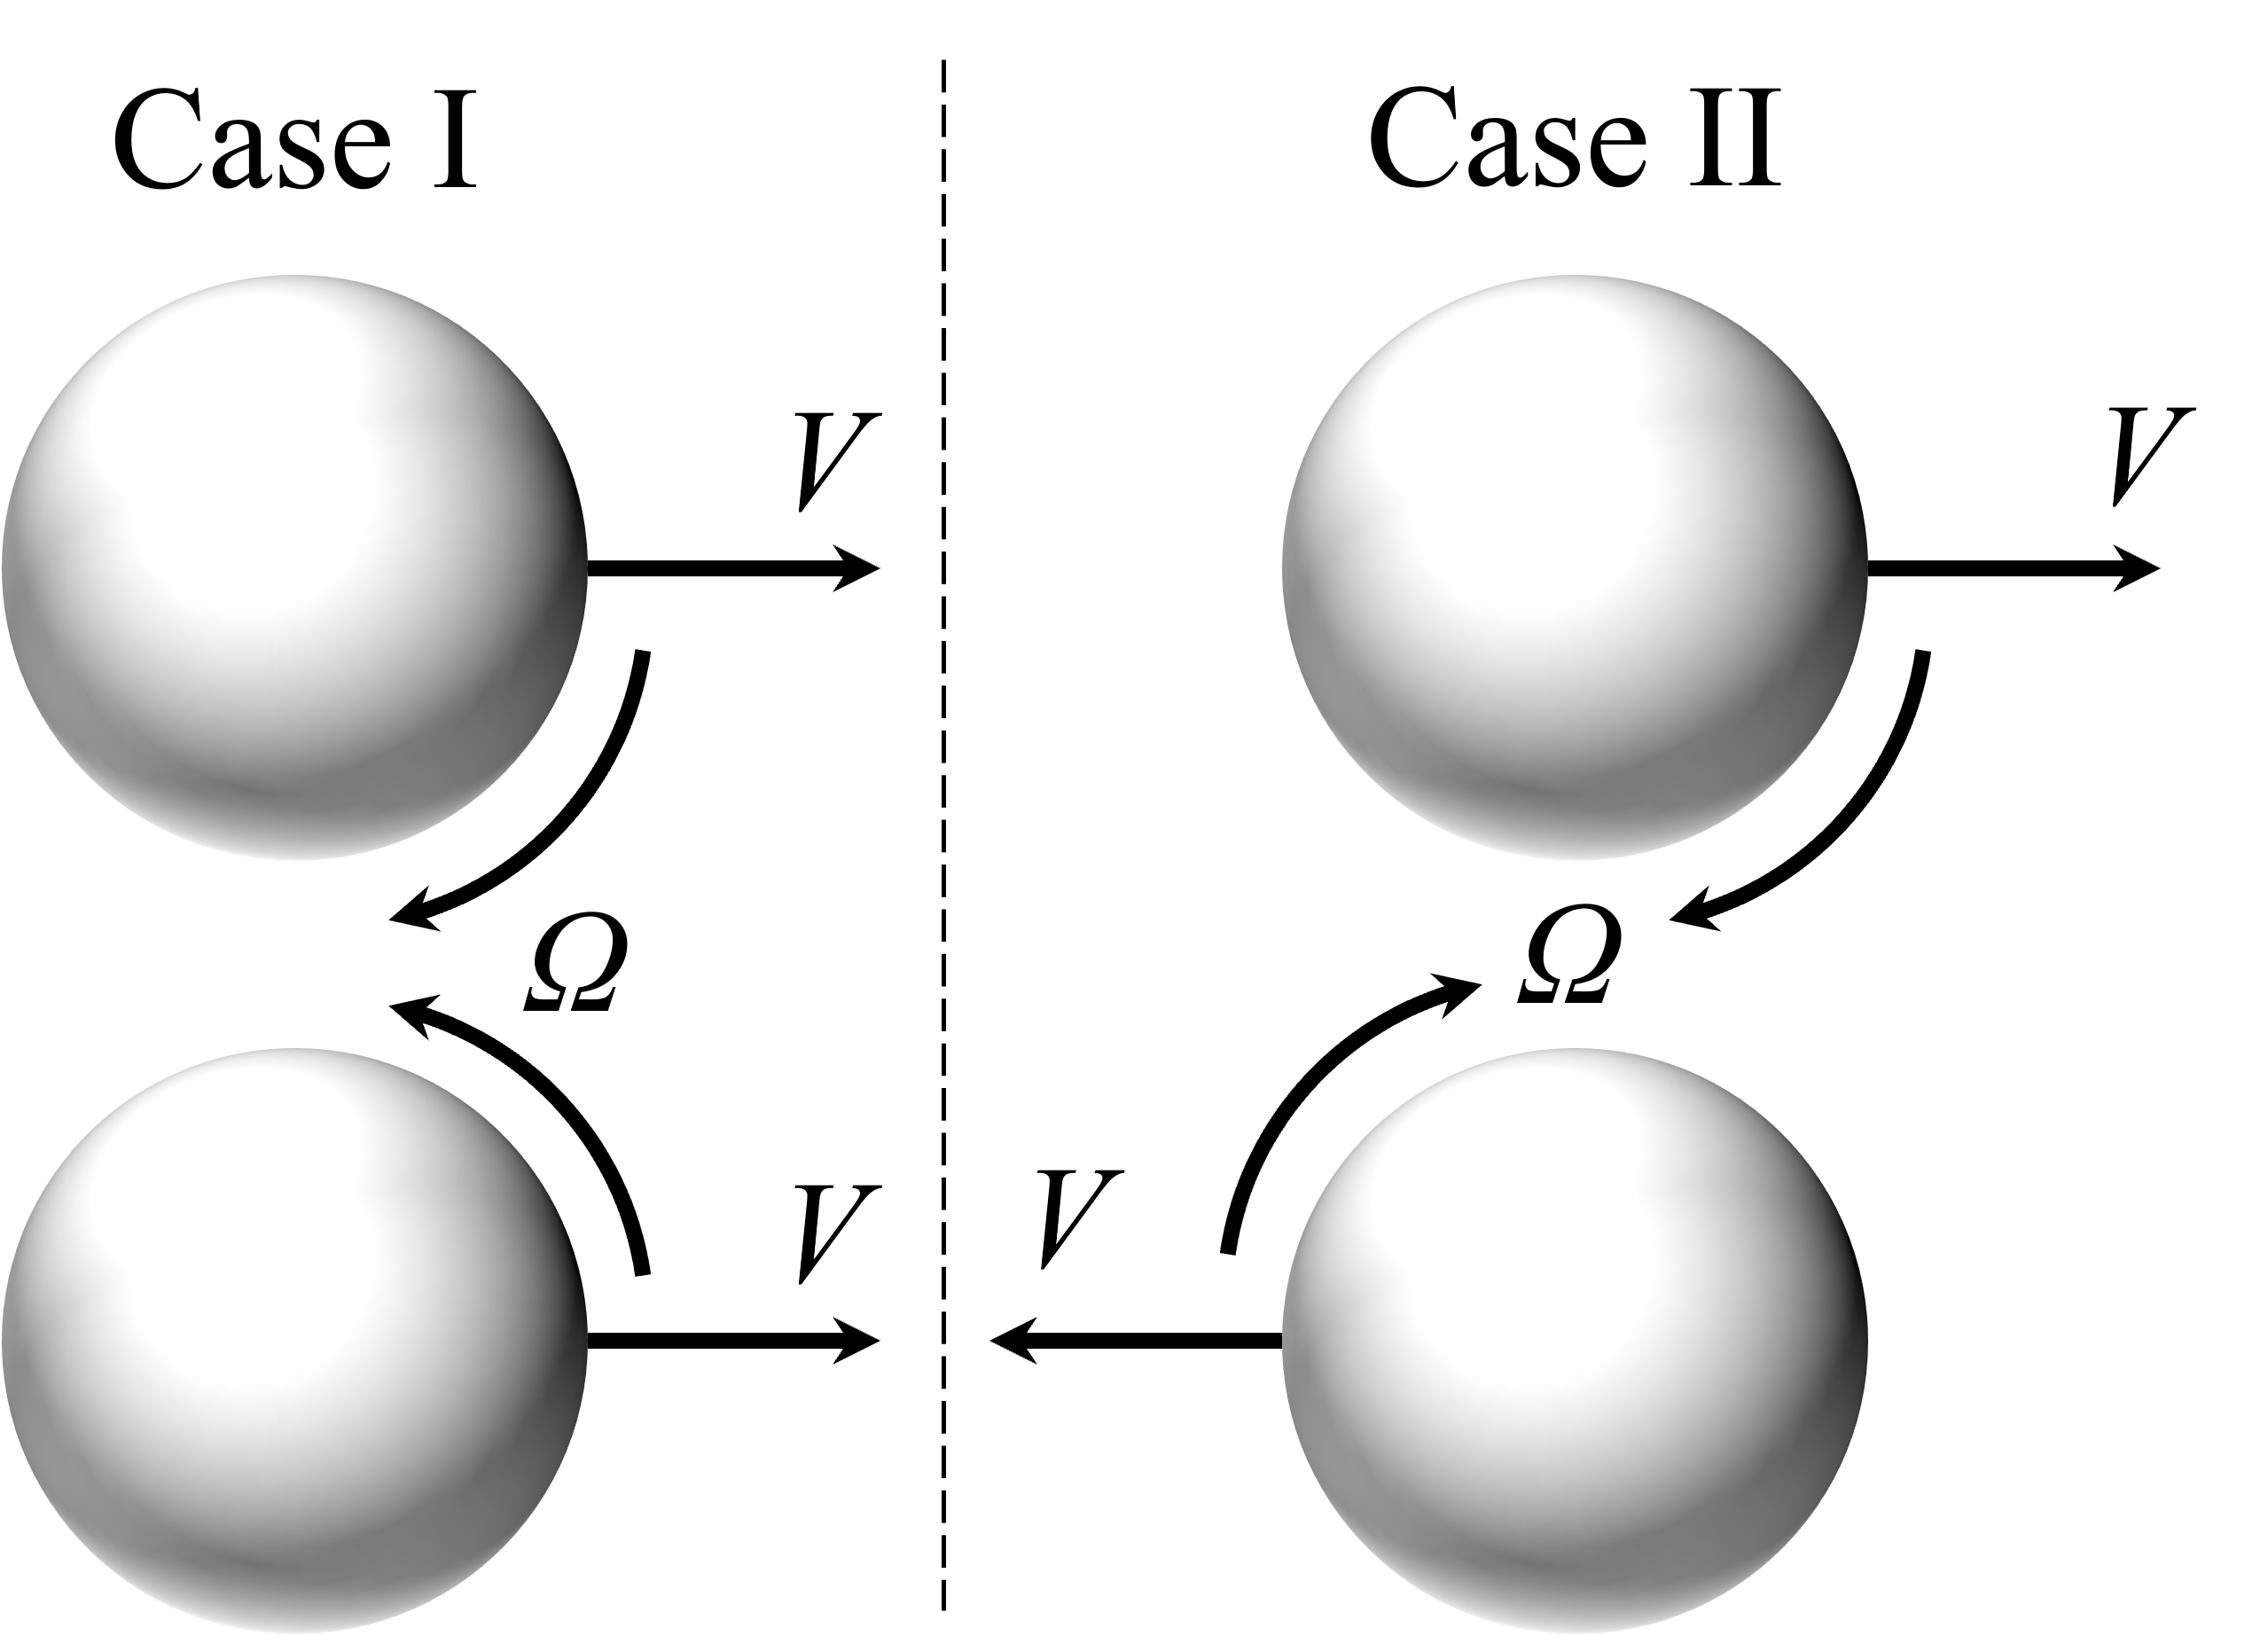
\includegraphics[trim=0mm 0mm 0mm 0mm, clip, width=0.6\textwidth]{../figs/PRF/fig2.png}
\caption{Two symmetric cases of free rotation for a rigid pair}
\label{fig:freerot}
\end{figure}
The drag force acting on a pair of spherical drops immersed in a viscous flow is a function of the viscosity ratio $\hat{\mu}_r$. When the viscosity of the fluid circulating inside the spheres greatly exceeds the viscosity of the external fluid, the dynamical properties (e.g.\ inertia) of these bodies become similar to those of rigid particles. In the limit of large $\hat{\mu}_r$, the drag forces predicted by the solution of \cite{WW72} approach those resulted from the analytical solutions developed for rigid spheres (e.g.\ \cite{SJ26}). For a pair of particles interacting normal to their line of centers, the solution for liquid spheres (e.g.\ \cite{Z80}) at high viscosity ratios corresponds to that of rigid particles (e.g.\ \cite{ONM70}) only in a particular case that the rigid pair is undergoing \textit{free rotation}. This was put forward by \cite{Z80} based on the solution he developed for the normal interaction of a pair of liquid spheres. According to that study, the moments of hydrodynamic forces about the centers of mass of spheres are always zero, even in the limit of high $\hat{\mu}_r$. Therefore, the forces acting on liquid particles in the limit of high viscosity ratios have to approach those due to translation of freely rotating rigid particles. This is because the net torque, i.e.\ sum of the torques caused by translation and rotation, acting on a pair of freely rotating rigid particles is zero.

A mathematical description of free rotation is presented here. Figure~\ref{fig:freerot} shows two cases for an identical pair of rigid spheres symmetrically translating with velocity $V$ perpendicular to their line of centers and rotating with $\Omega$ about their central axes that are normal to their line of centers. In both cases, if the torque due to translation is counterbalanced by an equal and opposite torque due to rotation, then the angular velocity $\Omega$ can be expressed in terms of translational velocity $V$ as follows
\begin{align}
\frac{T}{-8\pi\mu a^2} = \hat{T}^\text{tr}V + \hat{T}^\text{ro}a\Omega = 0 \implies a\Omega = -\frac{\hat{T}^\text{tr}}{\hat{T}^\text{ro}} V. \label{eq:free}
\end{align}
Consequently, the net force due to translation and rotation would be
\begin{align}
\frac{F}{-6\pi\mu a} = \hat{F}^\text{tr}V + \hat{F}^\text{ro}a\Omega = \left(\hat{F}^\text{tr}-\hat{F}^\text{ro}\frac{\hat{T}^\text{tr}}{\hat{T}^\text{ro}}\right) V, \label{eq:freerot}
\end{align}
which is smaller than $\hat{F}^\text{tr}V$ -- the force which would exist if the particles were merely translating, e.g.\ when rotation is neglected. Here, $\hat{F}$ and $\hat{T}$ are nondimensional resistance coefficients for equal pairs \citep{GCB66,ON69}. Note that the translational and rotational orientations of the pair differ, namely, if the pair is translating with equal velocities in the same direction, the angular velocities are equal but have opposite signs, and vice versa. Such a simple description is possible only when the problem is symmetrical, which means the spheres have the same radius and move with equal translational and rotational velocities. In a more general case, i.e.\ when the particles have different radii and different velocities, the resistance coefficients $(\hat{F}_i,\hat{T}_i)$ and consequently the forces and torques $(F_i,T_i)$ acting on them are not identical.



\subsubsection{Comparison of force representations}%%%%%%%%%%%%%%%%%%%%%%%%
In the step preceding the computation of the collision efficiency, a detailed comparison of different representations for the aerodynamic forces is made. The analysis concerns the relative motion of two spheres with equal and unequal radii. Two different cases are considered where the liquid spheres move at the same velocity in directions normal and parallel to the line connecting their centers. Figures~\ref{fig:models} to \ref{fig:fluidy} show interaction forces normalized by the Stokes drag acting on a single droplet for a wide range of normalized gap sizes, $\xi$.
\begin{figure}%fig:models_fig:models_fig:models_fig:models
\center
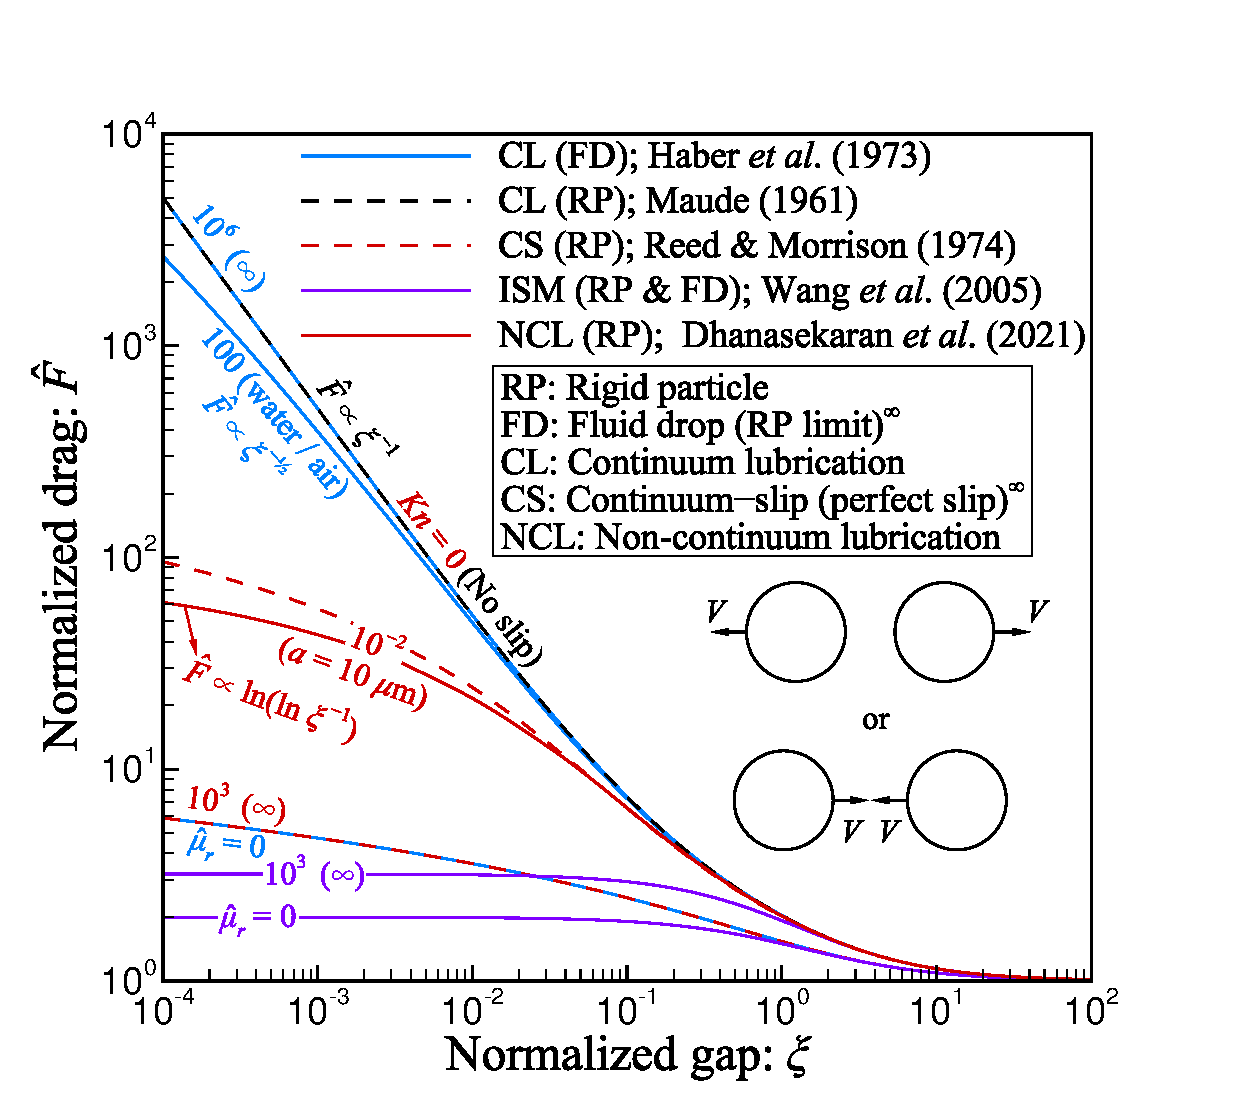
\includegraphics[trim=05mm 00mm 20mm 15mm, clip, width=0.6\textwidth]{../figs/PRF/fig3.pdf}
\caption{Comparison of the normalized aerodynamic force (resistance) acting on a pair of equal-size spherical drops moving with the same velocity but an opposing orientation along their line of centers. The approximate value (order) for the limit of each solution is marked with $\infty$, indicating an insignificant change for a larger $\hat{\mu}_r$ or $Kn$.}
\label{fig:models}
\end{figure}%%%%%%%%%%%%%%%%%%%%%%%%%%%%%%%%%%%%%%%%%%%%%%%%%%%%%
Figure~\ref{fig:models} shows the normalized drag force acting on an equal-sized pair of spheres moving with the same velocity in opposite directions along their line of centers. Such a comparison enables us to quantify distinctions in different formulations of aerodynamic forces, i.e.\ rigid particles under continuum or non-continuum lubrication, fluid drops, etc. The growth rate of each representation is shown next to the curves as $\xi \to 0$, that is the slope of the line for small $\xi$. Similar to rigid spheres, the resistance coefficients for a pair of fluid drops at large viscosity ratios (blue lines) increase to infinity but the growth rate, $\xi^{-1/2}$, is slower at moderate viscosity ratios \citep{Z78,DSR89}. These rates for the limiting cases of highest and lowest viscosity ratios, i.e.\ $\hat{\mu}_r \to \infty$ and $0$, approach $\xi^{-1}$ and $\sim0$, respectively. The former is consistent with the solution that assumes no-slip boundary condition on the surfaces of rigid spherical particles. The latter is quantitatively identical to the case of rigid particles under perfect slip \cite[lower red dashed line:][]{RM74}. Non-continuum lubrication force (red line) starts to deviate from both the continuum one (black dashed line) and the continuum--slip one (higher red dashed line) for $\xi<10^{-1}$. For larger separation distances the differences are negligible. There are two key differences in the representation of the drag force for a non-continuum flow in the gap. First, the growth rate as $\xi \to 0$ is weaker with $\hat{F}\propto\ln(\ln \xi^{-1})$ \citep{SK96,DRK21a}. Second, the value of this lubrication force is smaller, and the reduction depends on the Knudsen number. In this analysis, the mean free path is constant, and equal to $l_m = 0.1~\mu \text{m}$; therefore $Kn$ is only a function of the size of the pair. In practice, the mean free path is inversely proportional to the ambient pressure \citep{J88}. This dependence should be taken into account when modeling convective clouds, as the atmospheric pressure decreases with altitude.

The strict comparison of different formulations of aerodynamic interactions between a pair of typical cloud droplets, i.e.\ $a=O(10~\mu \text{m})$ and $\hat{\mu}_r=O(100)$, has been made with a rigid pair under no slip. The comparison reveals that the non-continuum effect has a much stronger influence on the reduction of lubrication forces than the mobility of interfaces of liquid particles. In other words, although each effect noticeably impacts lubrication forces, a combined description of both effects using the solution developed by \cite{RSD22} would be close to the continuum--slip one. Finally, the drag forces approximated by the ISM for two limits of viscosity ratio are shown. The two purple lines in Figure~\ref{fig:models} represent the interacting force for a rigid pair, i.e.\ when $\hat{\mu}_r\to\infty$ (rigid particle limit) and for a fluid pair with $\hat{\mu}_r=0$ (inviscid bubble limit). Both functions flatten for $\xi<10^{-2}$ suggesting that under the ISM, it is not feasible to accurately represent the short-range lubrication. Note that the resistances with $\hat{\mu}_r=0$ are presented only to show the limit of each representation, but they are not relevant to cloud droplets.

\begin{figure}%fig:nclmodel_fig:nclmodel_fig:nclmodel_fig:nclmodel
\center
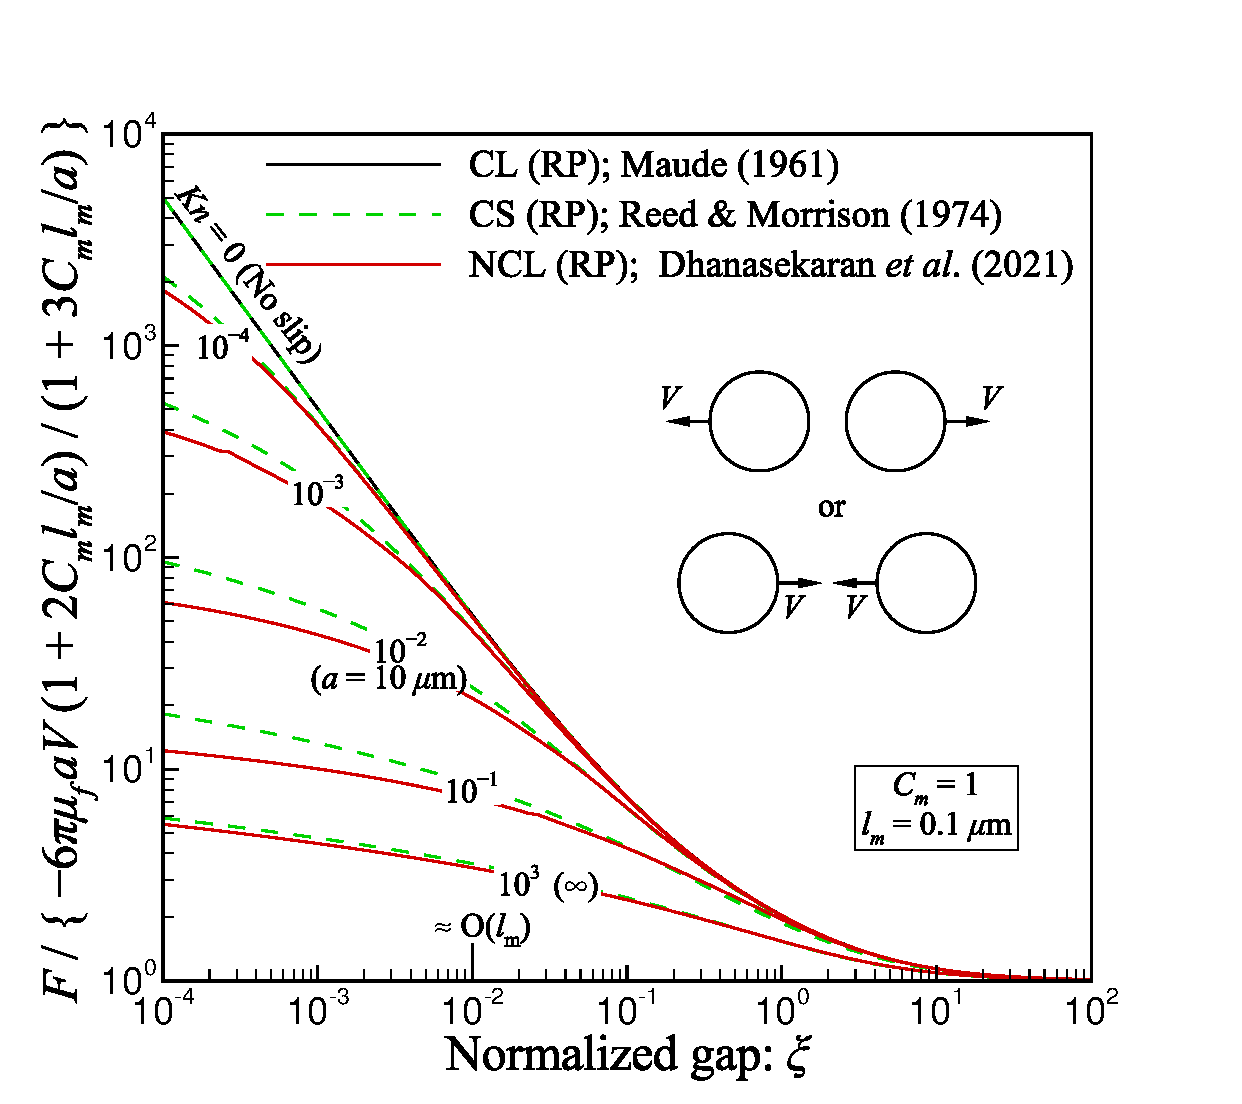
\includegraphics[trim=05mm 00mm 20mm 15mm, clip, width=0.6\textwidth]{../figs/PRF/fig4.pdf}
\caption{Comparison of drag forces acting on two rigid spheres that move along the line connecting their centers. The forces were evaluated at different $Kn$ using two different approaches: (i) continuum flow with slip boundary condition; (ii) non-continuum lubrication.}
\label{fig:nclmodel}
\end{figure}%%%%%%%%%%%%%%%%%%%%%%%%%%%%%%%%%%%%%%%%%%%%%%%%%%%%%%


Figure~\ref{fig:nclmodel} shows the normalized drag acting on two approaching rigid particles and quantify the differences resulting from considering the non-continuum effects. These drag forces are evaluated for a system with two equal-sized spheres at different Knudsen numbers, corresponding to different radii. The curves compare the standard solutions that assume continuity of the medium (black line) to those with non-continuum assumptions. The continuum--slip resistance (green dashed lines) is derived analytically assuming continuity of flow in the gap and having Maxwell slip boundary condition on particle surfaces. In the calculations we used $l_m = 0.1~\mu$m and $C_m=1$ \citep{D72}. This representation is valid when the gap is much larger than the mean free path of air molecules, and hence is limited to small Knudsen numbers ($Kn<0.1$). In addition, non-continuum lubrication force (red lines) evaluated analytically at different non-continuum regimes (including slip-flow) is shown, which is also valid at large $Kn$. The comparison shows how the non-continuum effects change the drag acting on rigid particles. For large separation distances the non-continuum representation \citep{SK96,DRK21a} agrees well with the continuum--slip solution of \cite{RM74}. This is because non-continuum lubrication of \cite{SK96} considers the slip flow for gaps much larger than the mean free path of molecules. Furthermore, all representations are identical in the limit $Kn=0$ for the entire range of the normalized gap. For small separations, however, the non-continuum lubrication deviates from the continuum--slip representation especially at larger $Kn$.

\begin{figure}%fig:modelssame_fig:modelssame_fig:modelssame
\center
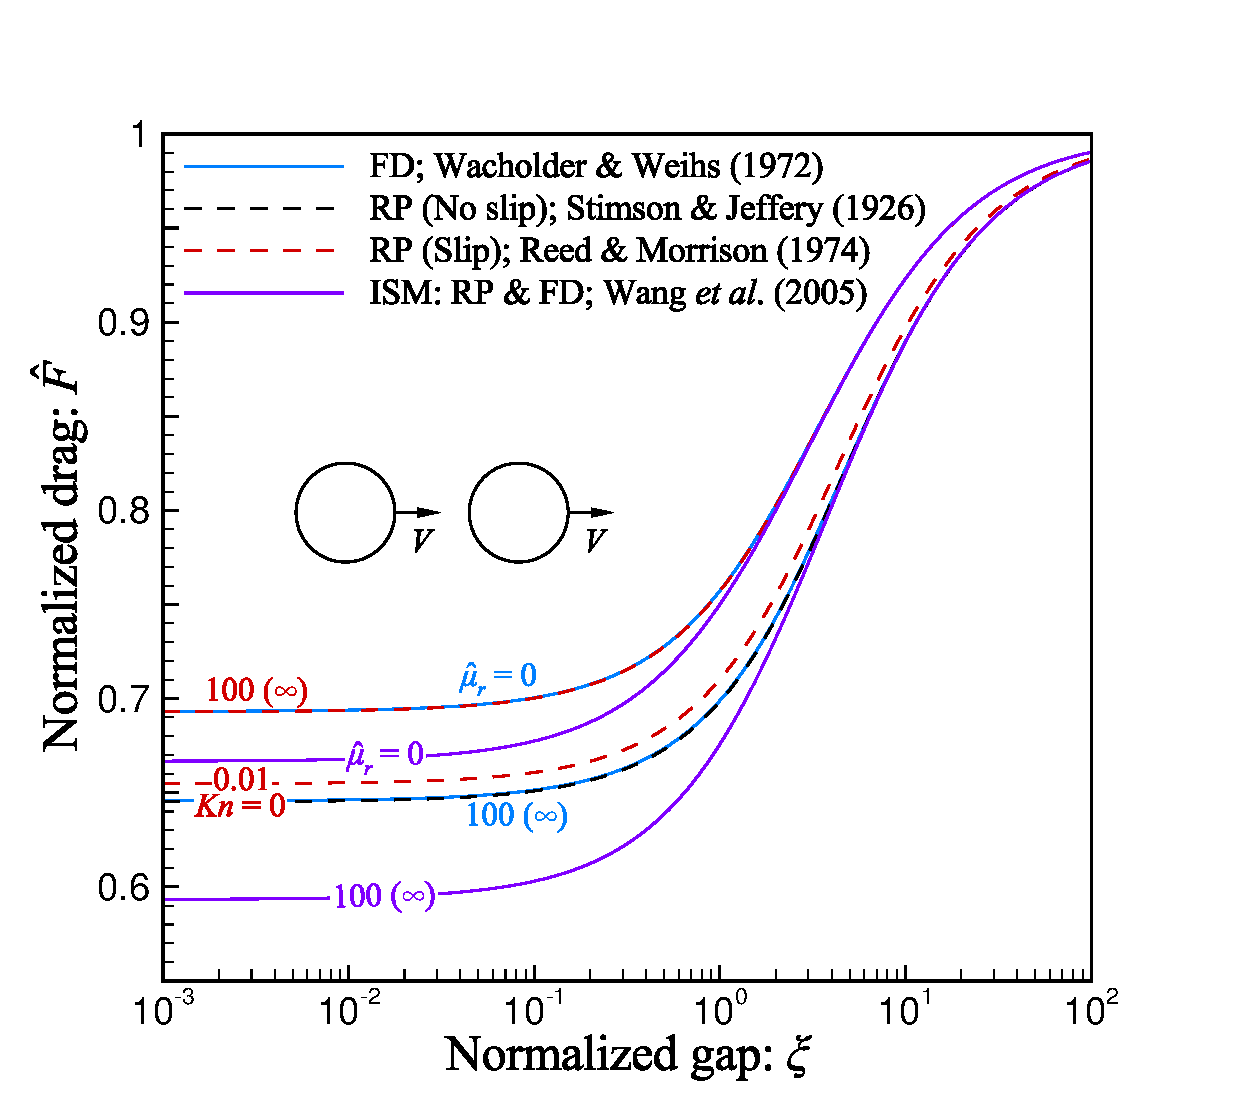
\includegraphics[trim=05mm 00mm 20mm 15mm, clip, width=0.6\textwidth]{../figs/PRF/fig5.pdf}
\caption{The drag acting on a pair of spheres translating in the same direction along their line of centers}
\label{fig:modelssame}
\end{figure}%%%%%%%%%%%%%%%%%%%%%%%%%%%%%%%%%%%%%%%%%%%%%%%
Figure~\ref{fig:modelssame} presents the normalized drag acting on a pair of spheres moving in the same direction parallel to the line of centers. As expected the force representation for a pair of fluid drops with $\hat{\mu}_r\to\infty$ is the same as that of rigid spheres without slip under the continuum assumption. A reduction in the viscosity ratio of a fluid pair enhances the drag until the limit $\hat{\mu}_r=0$. In this extreme case, the interactions between liquid particles and rigid particles under perfect slip are identical. The approximate representations from the ISM are also presented at the same limits $\hat{\mu}_r\to\infty$ and $0$, which can be compared with the exact representations (lower and higher blue lines, respectively).

In simulations here, depending on $Kn$ of each pair, the non-continuum effects for this type of motion is handled using the continuum--slip resistances of \cite{RM74} since, as mentioned, the solution by \cite{DRK21a} has been developed for an opposing orientation. When computing the collision efficiency of cloud droplets, this case is of particular importance. Small differences in the lubrication forces may result in large variations in $E_{12}$. The reason is that the velocity at which the droplets follow each other is relatively large and roughly proportional their terminal velocities. In the former case, i.e.\ squeezing flow, the relative velocities are definitely smaller and proportional to the differences in the terminal velocities.

\begin{figure*}%fig:fluidy_fig:fluidy_fig:fluidy_fig:fluidy
\center
{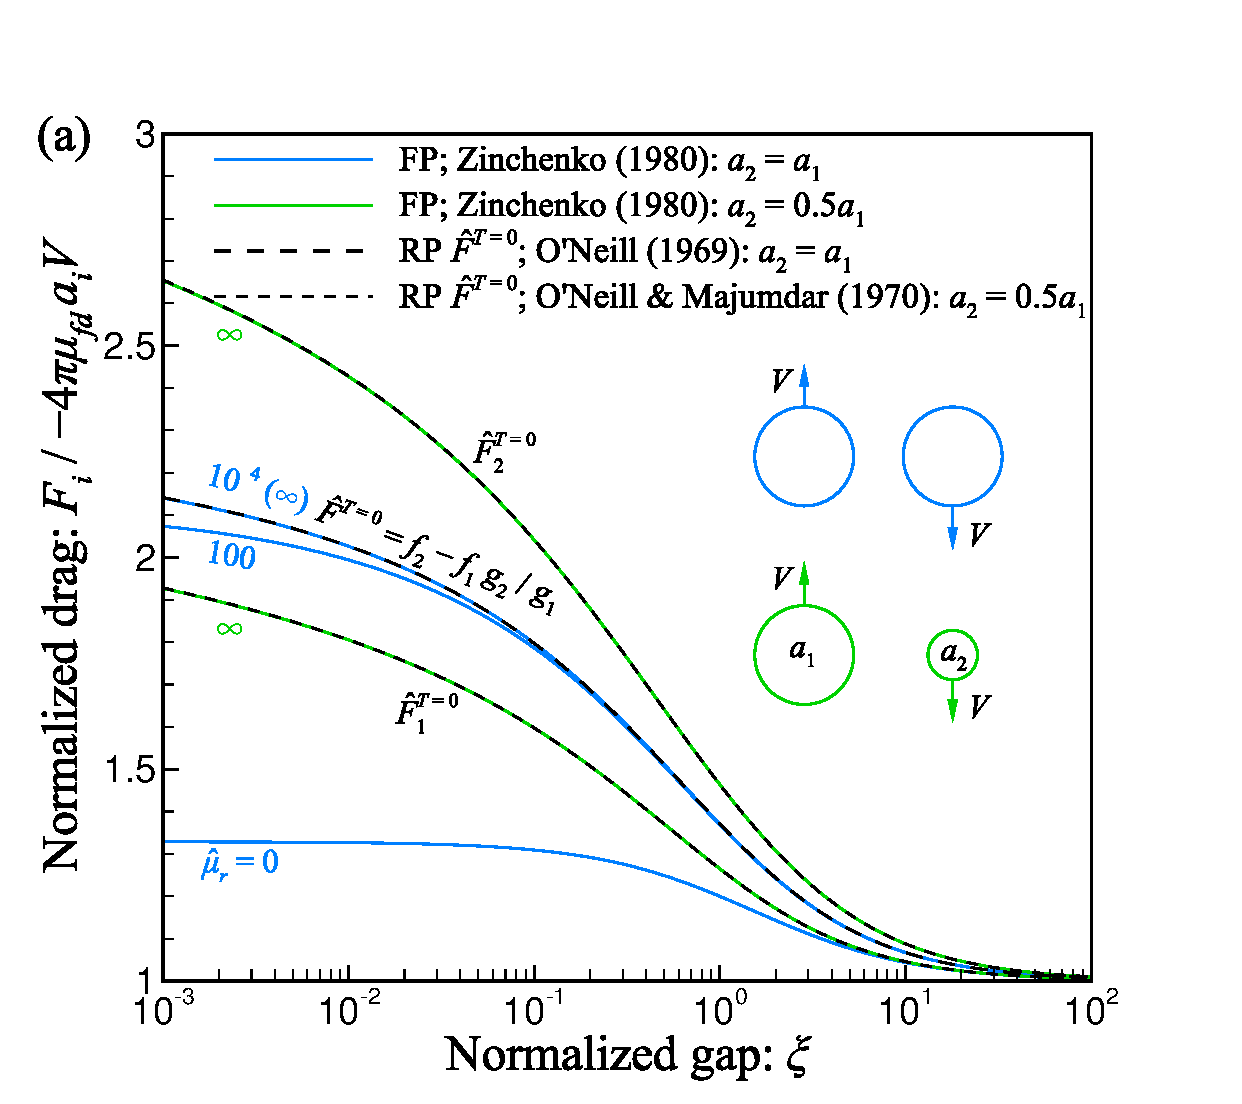
\includegraphics[trim=05mm 00mm 20mm 15mm, clip, width=0.48\textwidth]{../figs/PRF/fig6a.pdf}
 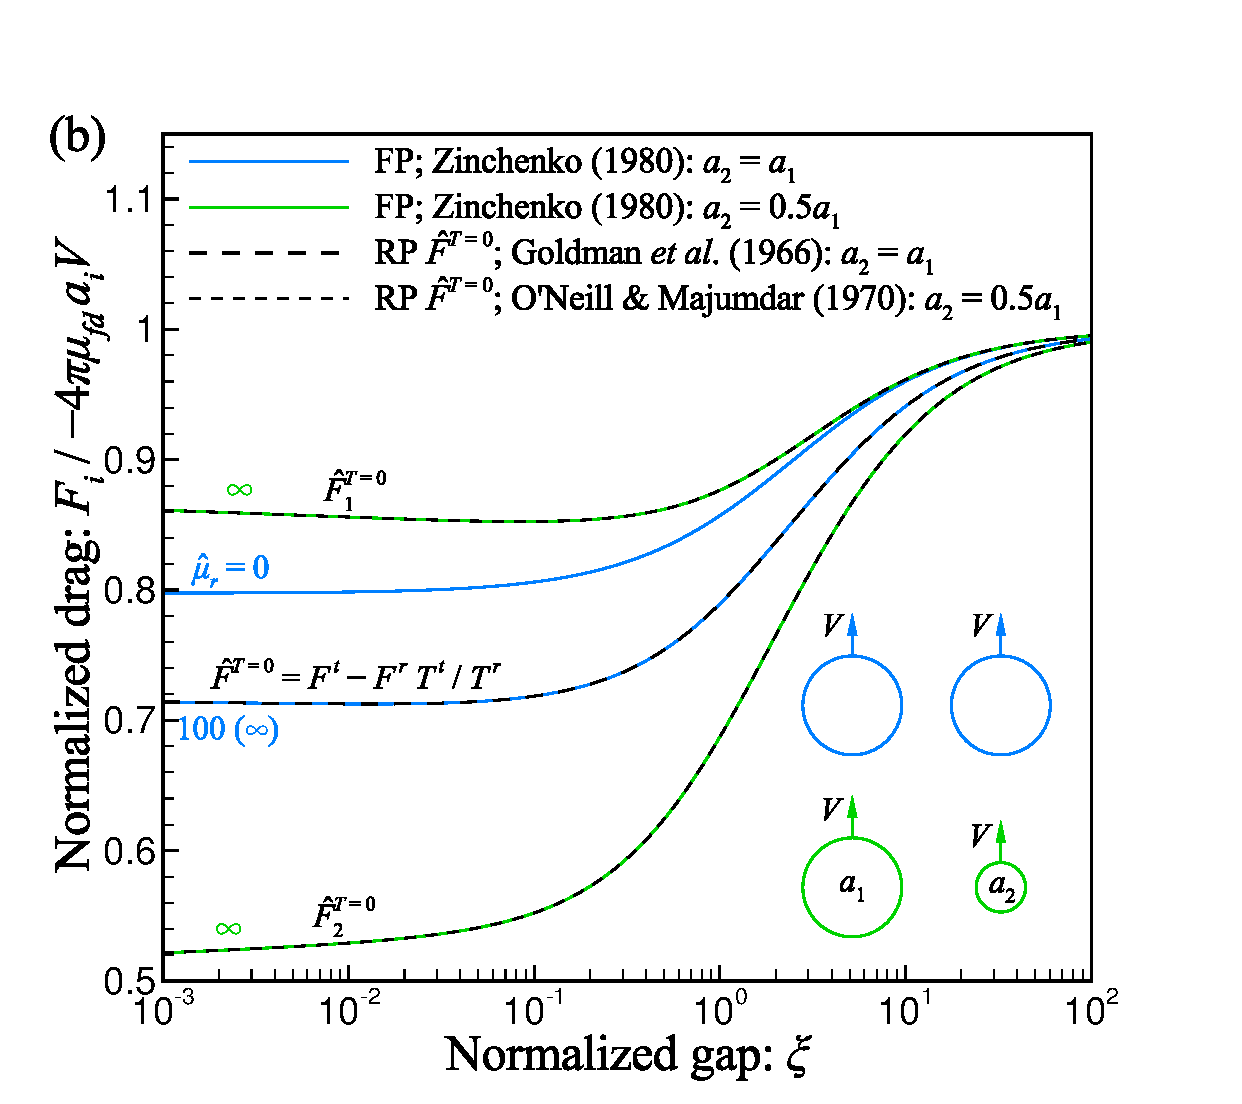
\includegraphics[trim=05mm 00mm 20mm 15mm, clip, width=0.48\textwidth]{../figs/PRF/fig6b.pdf}}
\caption{Comparison of the normalized drag acting on a pair of spheres translating normal to their line of centers in an (a) opposing or (b) the same direction. The two expressions for $\hat{F}^{T=0}$ follow the notations in each corresponding study.}
\label{fig:fluidy}
\end{figure*}%%%%%%%%%%%%%%%%%%%%%%%%%%%%%%%%%%%%%%%%%%%%%%

Further analysis concerns aerodynamic interactions of particles moving normal to their line of centers. Figure~\ref{fig:fluidy}(a) and (b) show the normalized drag acting on two equal and non-equal spheres moving in an opposite and the same directions, respectively. For a pair of fluid drops with equal radii (blue lines), the drags change with the viscosity ratio until reaching their limits. At this extreme value, the drag has an identical representation as the drag acting on a pair of freely rotating rigid spheres (black long-dashed line). The expressions for $\hat{F}^{T=0}$ shown in Figure~\ref{fig:fluidy} are the same as Equation~(\ref{eq:freerot}). The notations differ as they are adopted from the corresponding studies by \cite{GCB66} and \cite{ON69}.

The drag force at the limit of high viscosity ratio is additionally presented for spheres with unequal radii (green lines). The representations are also in accord with the net forces acting on an unequal pair of freely rotating rigid spheres (black short-dashed lines). For the comparison we used the solution developed by \cite{Z80}.


\subsection{Collision efficiency of a pair of droplets settling in quiescent air}
\begin{figure*}%fig:E12_E12_E12_E12_E12_E12_E12_E12_E12_E12
\center
{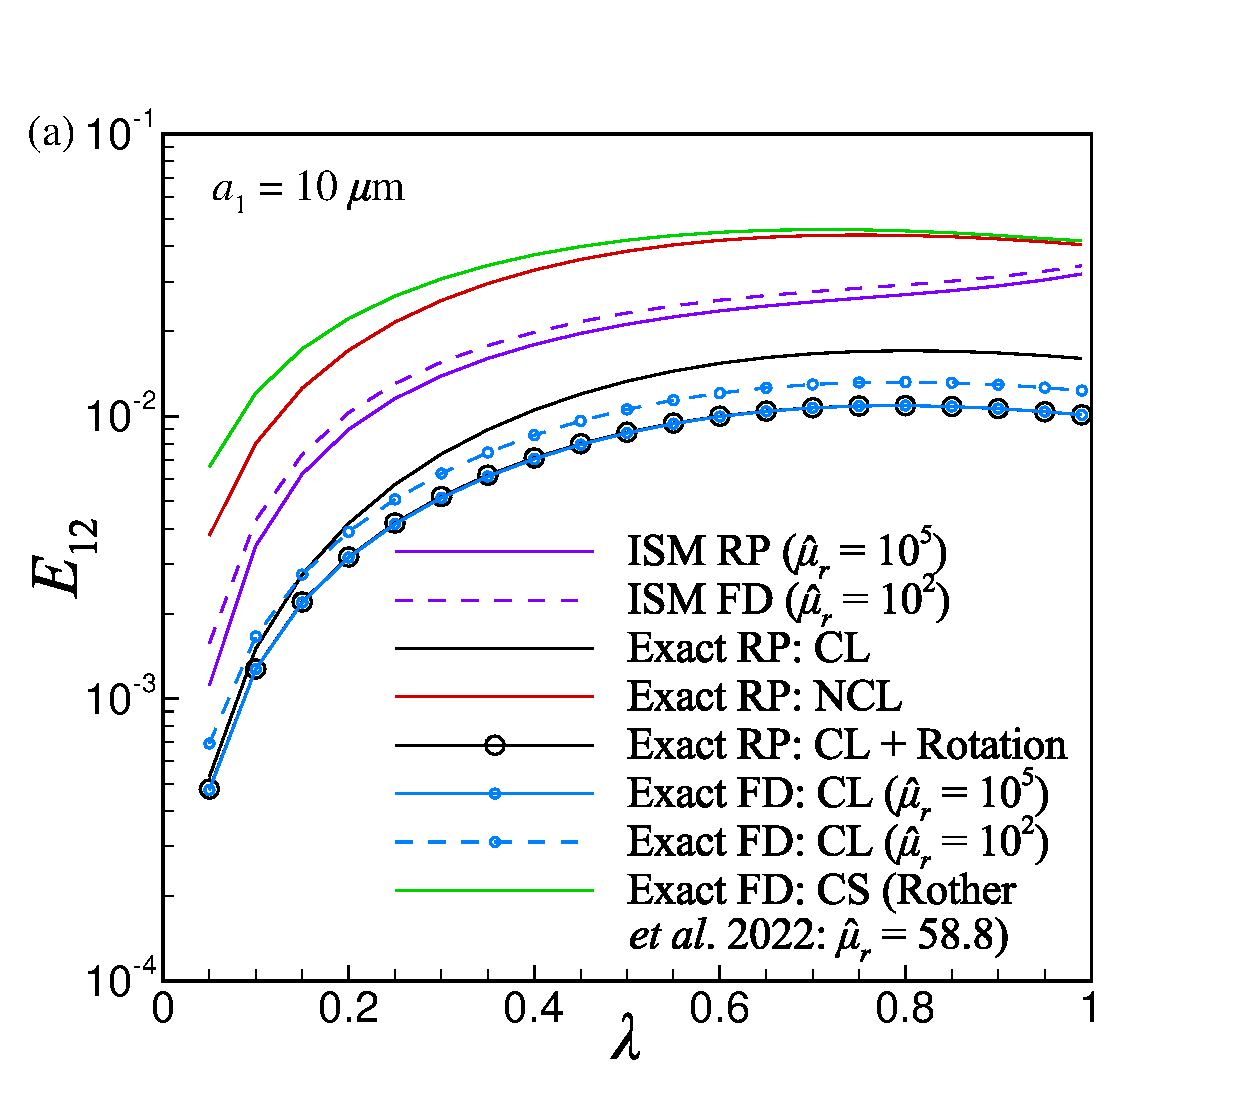
\includegraphics[trim=05mm 05mm 20mm 15mm, clip, width=0.48\textwidth]{../figs/PRF/fig7a.pdf}
 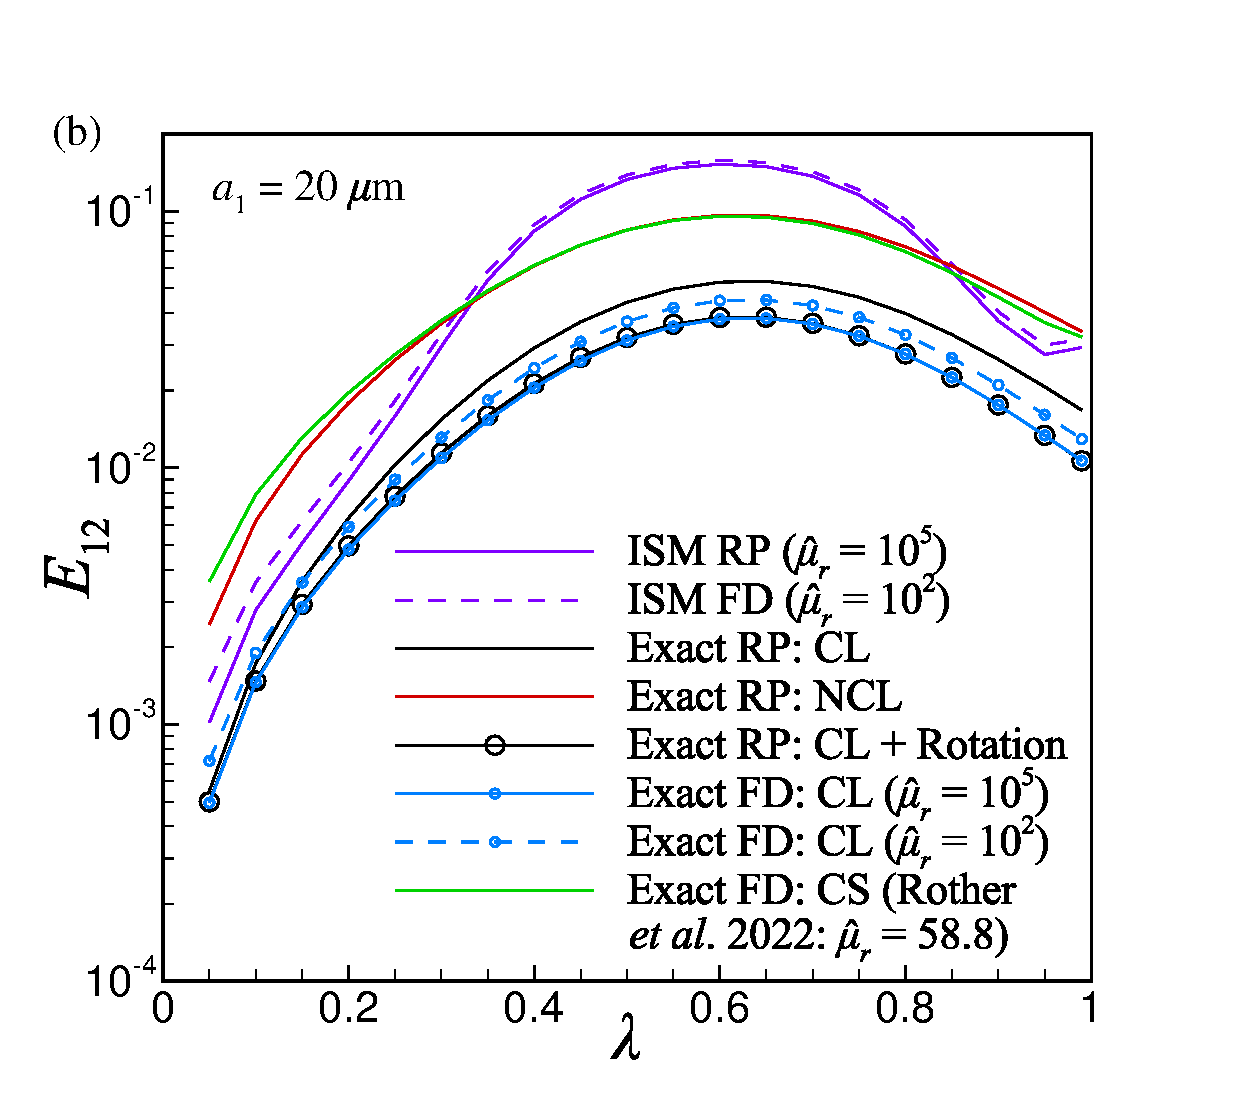
\includegraphics[trim=05mm 05mm 20mm 15mm, clip, width=0.48\textwidth]{../figs/PRF/fig7b.pdf}}
 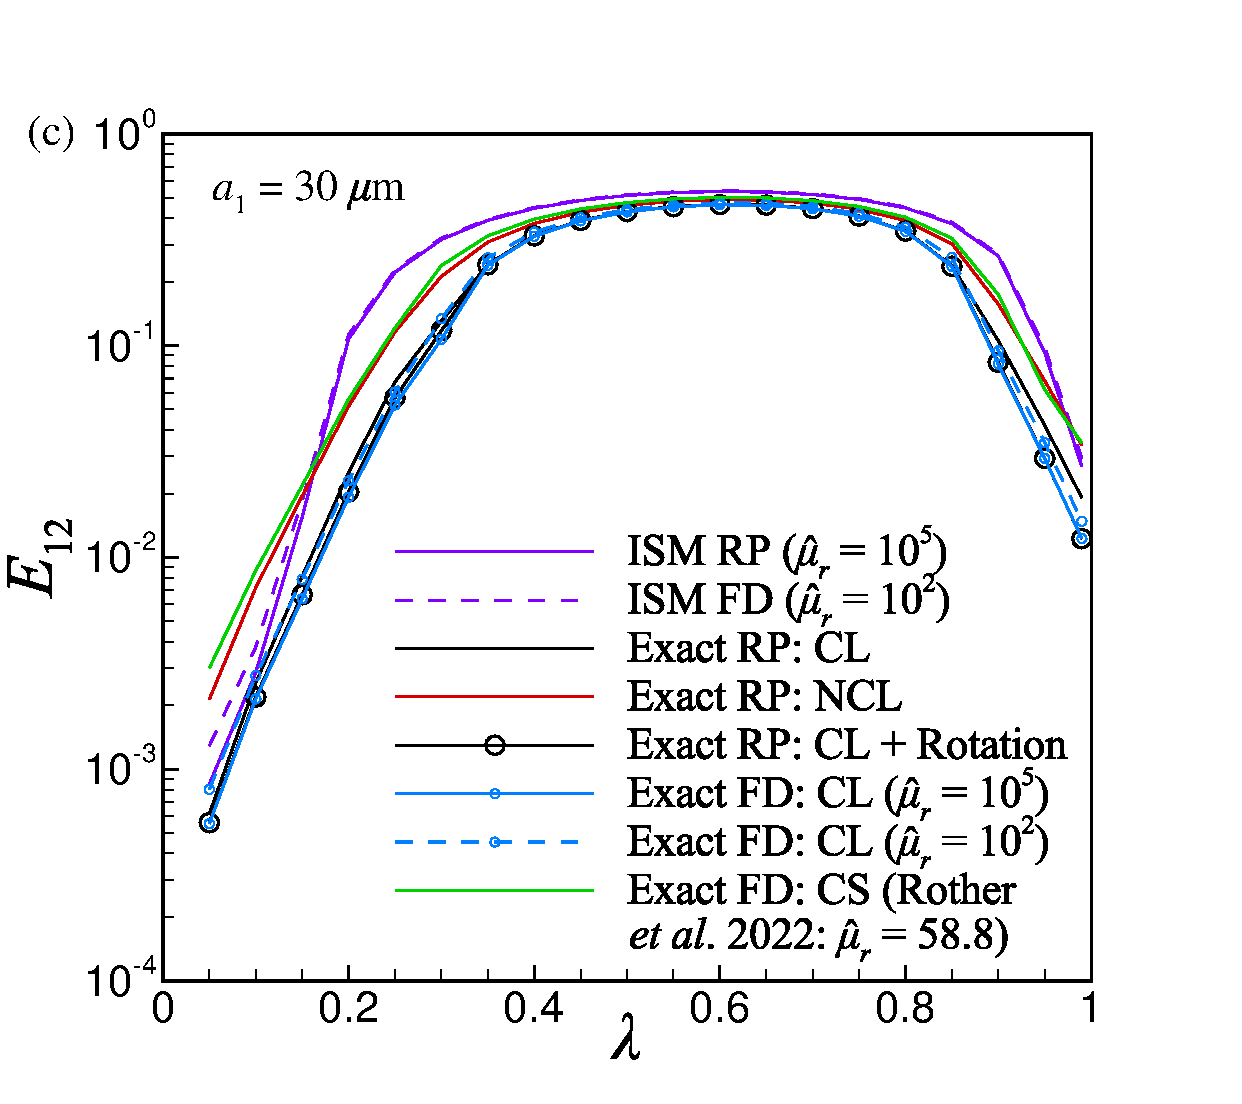
\includegraphics[trim=00mm 05mm 25mm 15mm, clip, width=0.48\textwidth]{../figs/PRF/fig7c.pdf}
\caption{Collision efficiency as functions of radius ratio under various force representations}
\label{fig:E12}
\end{figure*}%%%%%%%%%%%%%%%%%%%%%%%%%%%%%%%%%%%%%%%%%%%%%%
The collision efficiency computed using different representations of aerodynamic forces discussed above is presented in Figure~\ref{fig:E12}(a)--(c). Three panels correspond to simulations with different radii of the larger droplets, namely $a_1=10, 20, 30~\mu$m. The radius of the smaller droplet depends on the parameter $\lambda$ -- specified on the horizontal axis. The effects of droplet inertia, radius ratio and van der Waals force have already been discussed in several former studies \citep{HJ70,D84,RWMG11}. Accordingly, van der Waals forces are not taken into consideration in the present simulations. Here, the main focus is on the impact of non-continuum lubrication and internal circulation of the water inside droplets (fluid pairs with mobile interfaces). The reference $E_{12}$ has been computed for a pair of rigid spheres under the continuum flow assumption using two different force representations: (i) resistance functions of \cite{JO84} and (ii) solutions in bispherical coordinates of \cite{SJ26} and \cite{ONM70}. Both methods give similar results and the difference is much less than 1\%. Therefore, in Figure~\ref{fig:E12}(a)--(c), only the results from \cite{JO84} representation is shown (black solid line), marked with ``Exact RP: CL.'' The raw numerical data are also tabulated in Appendix \ref{sec:E12} -- Tables \ref{tab:E10}, \ref{tab:E20}, \ref{tab:E30}. In all three panels, $E_{12}$ computed under the exact force representation (black solid line) agrees well with results of \cite[][Figure 3]{HJ70}. Also, $E_{12}$ evaluated using the ISM for a rigid pair matches well the data in \cite[][Figure~8 and Table~5]{WAG05}. A slight discrepancy is, among other factors, due to the different definitions for the collision gap. A common method to avoid the problem of drag singularity is a tiny enlargement of the collision radius. 
This is usually done by increasing the radius of the \textit{larger} particle, such that the new collision radius is $R_\text{col}=R+\epsilon_\text{col}a_1$ \citep{HJ70,WAG05,RWMG11}. However, in the analysis presented here the minimum separation distance below which the collision is assumed is a fraction of the \textit{average} radius: $R_\text{col}=R(1+\tfrac{1}{2}\xi_\text{col})$ where $\xi_\text{col}=10^{-3}$.

The colors, marks, and patterns of curves are chosen to make comparison more convenient. The purple lines represent $E_{12}$ computed using the ISM. The colors black and blue correspond to the models for rigid particles and fluid drops, respectively. The blue lines are marked with circles to be compared with the circle-marked black line that takes the rotation of rigid particles, Equation~(\ref{eq:eqm3}), into consideration. The red line marks the simulations that account for the non-continuum effects in lubrication forces. The green line shows a particular case from the reference data of \cite{RSD22} in which the van der Waals forces are excluded. As such, the data can be fairly compared with the models utilized here. These collision efficiencies \citep{RSD22} are computed using a model through which the internal circulation and non-continuum effects (within free-slip regime) are jointly accounted for. The differences between the rigid particles and fluid drops are manifested using different values of the viscosity ratio, which are $\hat{\mu}_r=10^5$ and $10^2$, correspondingly. The latter corresponds to the water droplets in air under typical conditions of atmospheric clouds. The black line with circle symbols is the only case in which the rotation of rigid pairs, Equation~(\ref{eq:eqm3}), is considered. Based on the obtained results, noticeable differences in $E_{12}$ are only observed for the droplets with low inertia (the two cases for $a_1=10$ and $20~\mu$m). For larger droplets, different force representation models predict similar values for the collision efficiency. 

The approximate force representation obtained from the ISM does not capture the singularity of the lubrication forces \cite[Figure~7(a) in][]{WAG05}. Therefore, the resistance remains finite when the gap between the droplets goes to zero. This allows us to compute $E_{12}$ even without employing the collision gap model, that is $R_\text{col}=a_1+a_2$. The differences in the collision efficiency between the rigid particles and fluid drops (solid vs.\ dashed purple line) are clearly visible for $a_1=10~\mu$m. Overall, $E_{12}$ of liquid drops is about 10\% larger. This is due to the lower drag force acting on a single liquid sphere compared to the rigid one. In general, the ISM largely overestimates $E_{12}$ when compared with the exact representation (purple vs.\ blue lines).

Under exact force representations for a rigid pair, $E_{12}$ is significantly larger when considering the non-continuum lubrication (red vs.\ black line). The relative increase due to non-continuum effects is more pronounced for smaller droplets, on average $\approx125$\%, see Figure~\ref{fig:E12}(a). For larger droplets this enhancement is about $25$\% (e.g.\ in panel (c) of Figure~\ref{fig:E12}) since higher inertia of these droplets has a stronger impact on collisions. The reason for the observed increase is the lower drag force acting on particles in squeezing flow. For two closely spaced rigid spheres approaching with equal velocities, the repulsive aerodynamic force evaluated under the continuum assumption is inversely proportional to the separation gap, i.e.\ $\hat{F}\propto\xi^{-1}$. However, if the non-continuum effects are accounted for, the drag takes a sluggish logarithmic growth, i.e.\ $\hat{F}\propto\ln(\ln\xi^{-1})$ \citep{SK96,DRK21a}. This estimate quantifies the dependency between lower drag and higher probability of collisions. Moreover, the results of \cite{RSD22} follow a similar trend to the results computed using the non-continuum lubrication model (green vs.\ red line). The resemblance is mainly due to the non-continuum lubrication effects, whereas the differences are caused by two important factors. Firstly, \cite{RSD22} developed a solution for a pair of fluid drops (having internal circulations with mobile interfaces), while \cite{DRK21a} considered rigid particles. Secondly, in each study non-continuum lubrication has been quantified in a different manner. To do so, \cite{RSD22} imposed slip boundary condition on drop surfaces while assuming a continuous flow in the gap between droplets. This is accurate at low $Kn$ as long as the gap is much larger than the mean free path of the flow. On the other hand, \cite{DRK21a} used several solutions obtained within various non-continuum regimes, which is valid at high $Kn$ and for gaps smaller than the mean free path of air molecules. Furthermore, it is worth adding that the less steep increase in the non-continuum lubrication forces enables performing simulations without having to use the collision gap model. This leads to a small ($\approx2\%$) decrease in $E_{12}$ (see Tables \ref{tab:E10} to \ref{tab:E30} in Appendix \ref{sec:E12}).

The next set of results, shown in Figure~\ref{fig:E12}(a)--(c) using circle-marked black line, presents $E_{12}$ computed in simulations that account for rotation of rigid particles. These values are in accord with $E_{12}$ for liquid particles with $\hat{\mu}_r=10^5$ (solid circle-marked blue line). This is an important finding viewing the fact that two different set of problems yield the same results. An unavoidable consequence of considering particle rotation is the significant increase of the computational complexity. Accounting for rotational motion requires the calculation of more quantities including torques, angular velocities, additional resistance functions (defining the coupling between translational and rotational motion), and modified drag forces. The ordinary differential equation governing the angular velocity of rigid particles, i.e.\ Equation~(\ref{eq:eqm3}), must be solved together with the equation for the translational velocity. All these factors remarkably enhance the computational time compared to the case in which rotation is neglected. As for the spherical drops, an equation for the angular momentum does not need to be solved since a rigid-body rotation is not defined for the internal flows circulating inside the droplets and the external torques acting on the droplets are zero. Thus, the computational time is much shorter while values of $E_{12}$ are in a quantitative agreement with those for the freely rotating rigid particles. The obtained results are consistent with the theory developed by \cite{Z80}. According to hypotheses formulated there, the forces acting on two liquid particles with a very large $\hat{\mu}_r$ translating \textit{normal} to their line of centers are equal to those due to the translation of freely rotating rigid particles (see Figure~\ref{fig:fluidy}). It is also worth adding that the forces acting on two fluid drops of large $\hat{\mu}_r$ translating \textit{along} their line of centers \citep{WW72,HHS73} are similar to those of rigid particles \citep{SJ26,M61,JO84}. For the problem considered here, the conditions guaranteeing the free rotation are satisfied, because (i) the initial condition imposed is $\Omega_i = 0$ and (ii) there are no external torques acting on the droplets.

In Figure~\ref{fig:E12}(a) and (b), comparison between rotating (circle-marked black line) and purely translating (regular black line) rigid pairs demonstrates that when the particles are allowed to rotate $E_{12}$ declines roughly by 10 to 30\% as $\lambda$ increases from the smallest to largest values. Rotation, via the coupling terms in the resistance matrix, modifies the net drag acting on the pair normal to the line of centers, thereby reducing the chance of collision.


\begin{figure}%fig:decomp_decomp_decomp_decomp_decomp_decomp
\center
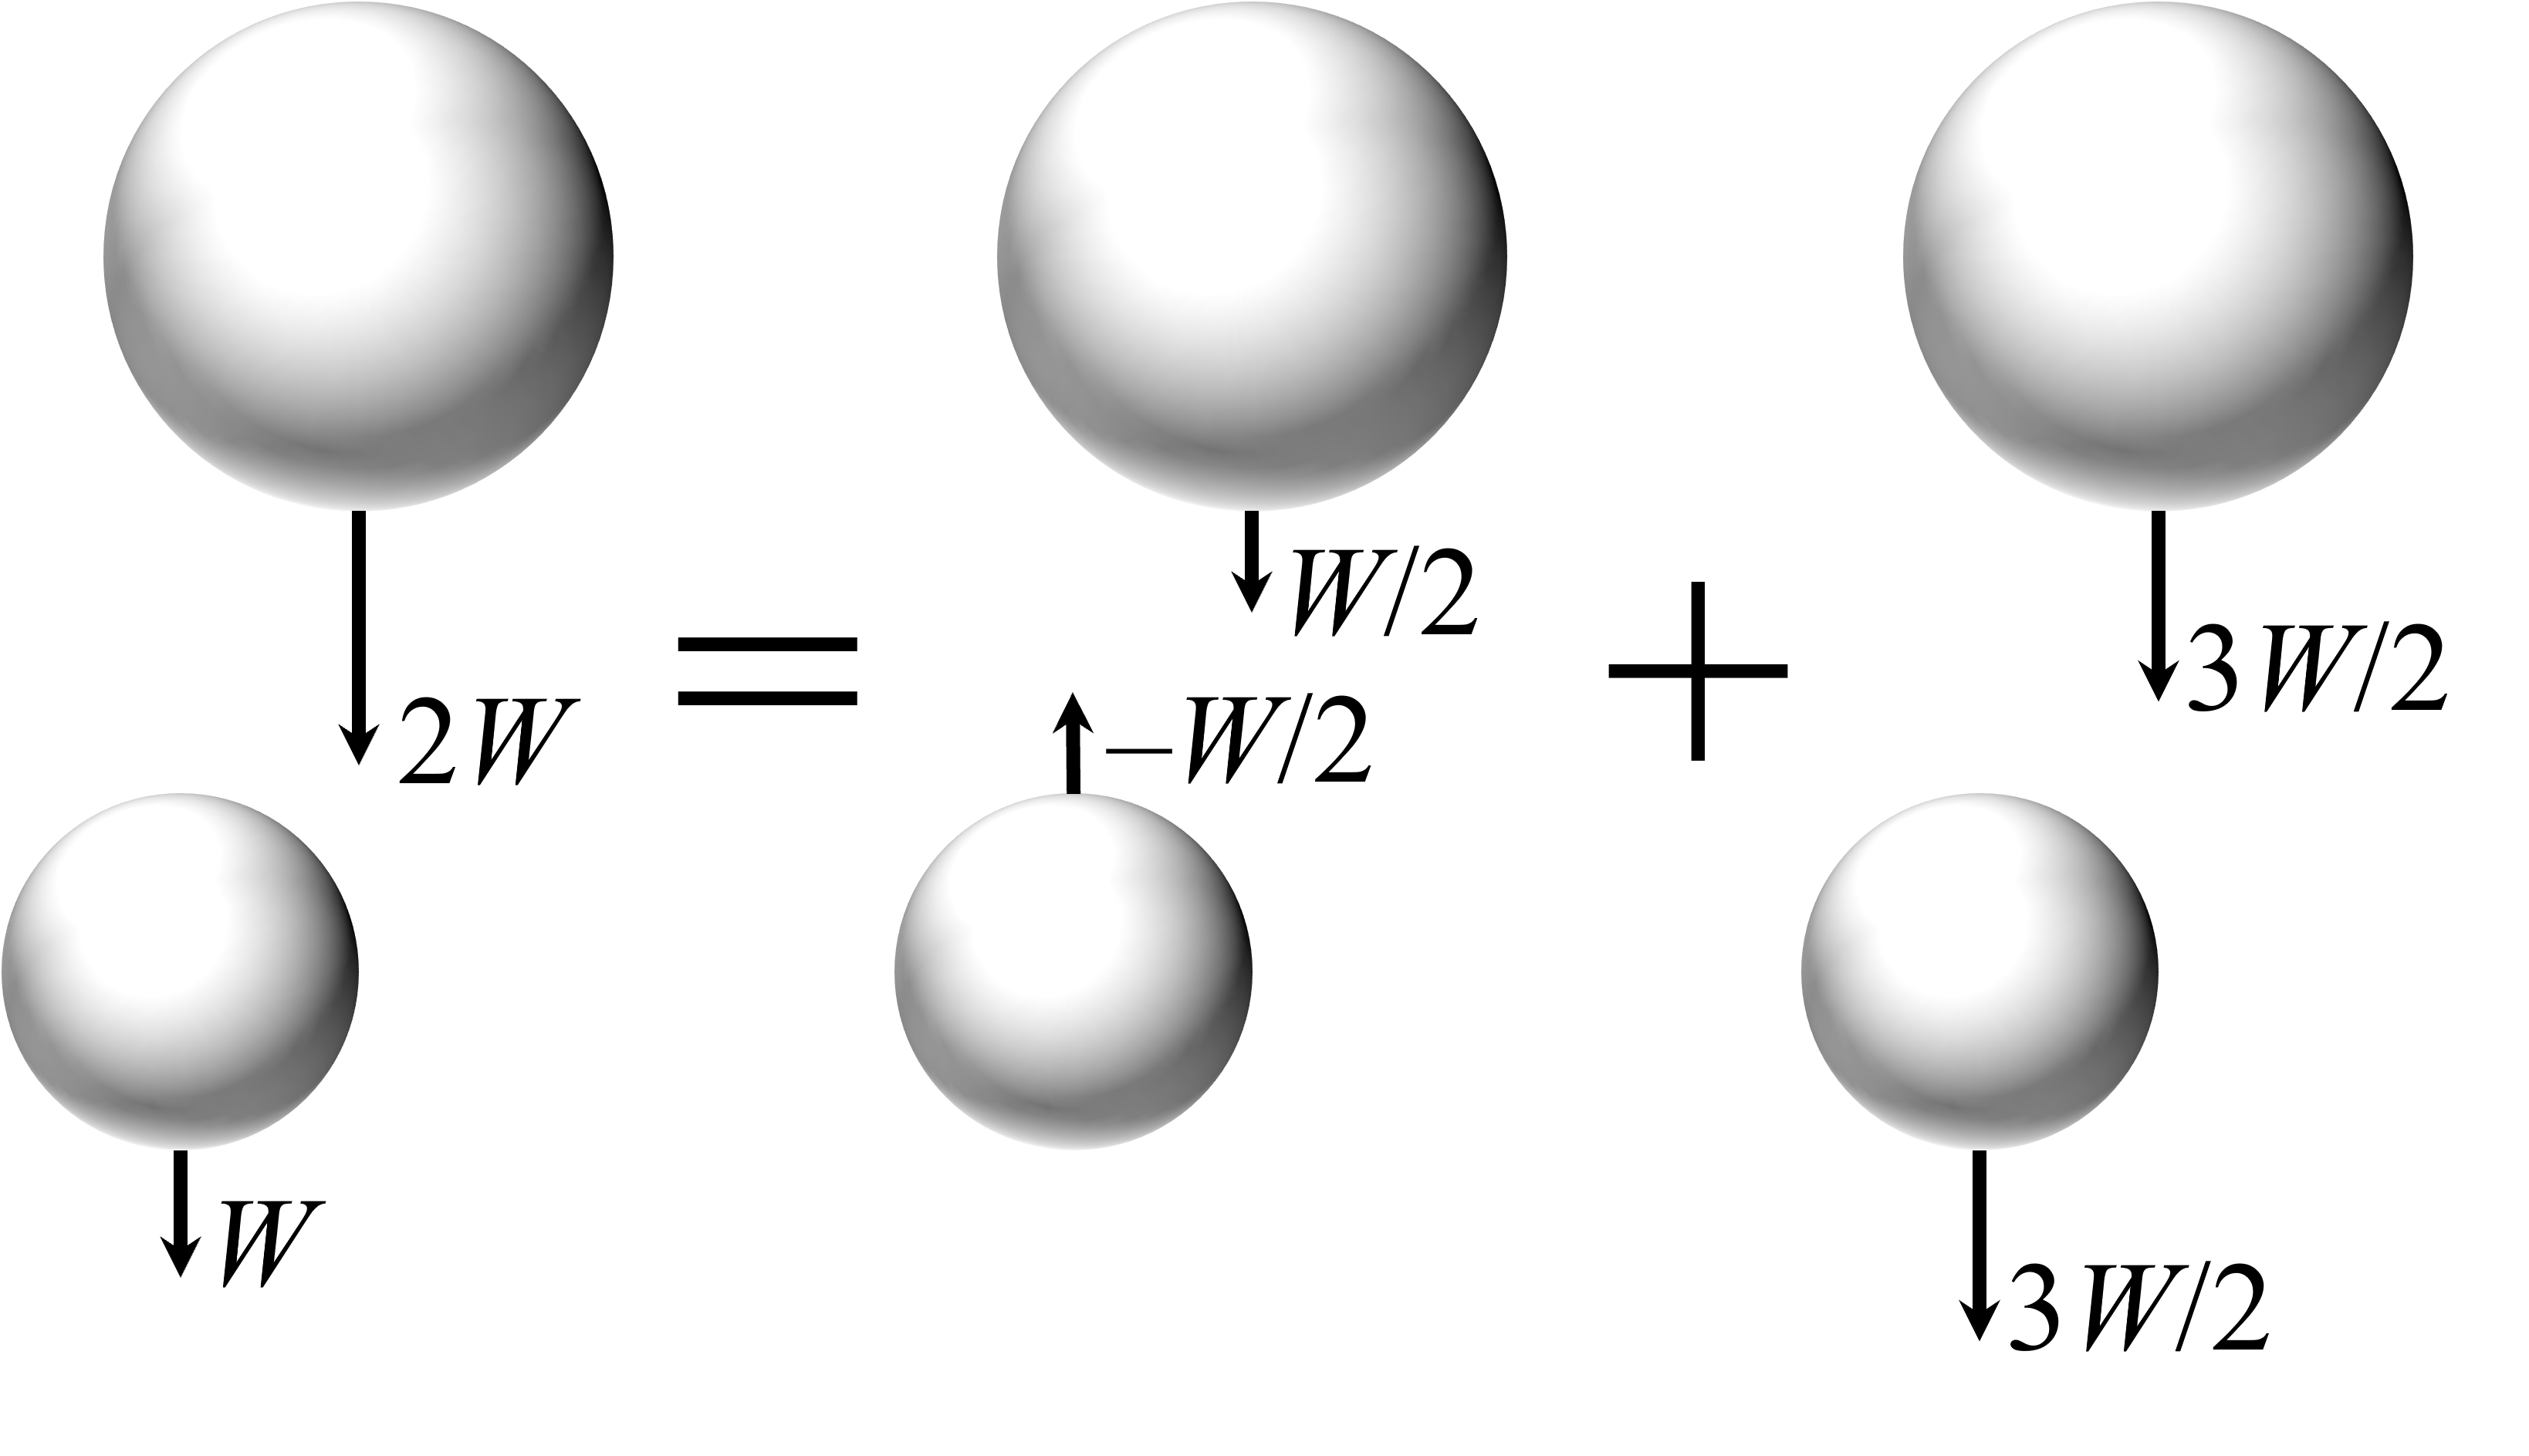
\includegraphics[trim=00mm 10mm 05mm 00mm, clip, width=0.6\textwidth]{../figs/PRF/fig8.png}
\caption{Decomposition of velocity of an arbitrary two-body system with $\lambda=0.7$ into two elementary and symmetrical cases.}
\label{fig:decomp}
\end{figure}%%%%%%%%%%%%%%%%%%%%%%%%%%%%%%%%%%%%%%%%%%%%%%%%
%
For a pair of water droplets in still air, the viscosity ratio is of the order of $\hat{\mu}_r = 10^2$. Under such conditions, the collision efficiency of water droplets (blue dashed line) is larger than that for freely rotating rigid particles of the same density or liquid particles at $\hat{\mu}_r = 10^5$. This enhancement is from $\approx20$\% for almost equal-sized ($\lambda\to1$) pairs to $\approx45$\% for the smallest radius ratio considered here ($\lambda=0.05$). Again, the reason for the increase in $E_{12}$ is the lower drag force acting on the approaching particles. We should be aware, however, that the comparison with purely translating rigid pairs (regular black line) is somehow biased because the interfaces (between drops' internal and external flows) of droplets are mobile.

Another comparison concerns the results obtained by employing exact and approximate (evaluated through the ISM) representations of aerodynamic interactions. One would expect that since the ISM yields a much smaller drag (at short separation distances) than non-continuum lubrication (see Figure~\ref{fig:models}), $E_{12}$ under the ISM has to be always larger. It turns out, however, that in many cases the trend is opposite (see Figure~\ref{fig:E12}(a) and (b)). The reason can be explained by considering a simplified example. For a pair of cloud droplets of radius ratio $\lambda = 0.7$, the terminal velocity of the smaller droplet is approximately half (since $\tau_i\propto a_i^2$) of the larger one. If aerodynamic interactions were neglected, the pair would maintain the same terminal velocities while settling under gravity. In Figure~\ref{fig:decomp}, these terminal velocities are decomposed (see Figure~1 in \cite{RWMG11}) into two elementary cases of the pair approaching and following at the same velocity. The first case on the RHS, based on exact solutions, is subjected to the singular resistances which prevent collision unless the collision gap model is utilized. For this case, a stronger drag reduces $E_{12}$. The second case on the RHS is also important for this problem since a major contribution to total velocity is due to the pair following each other along gravity. (The least effective cases would be related to the horizontal components of velocities, being zero here, since they would be much smaller than settling velocities if aerodynamic interaction were considered.) For the second case, slight variations in the drag forces significantly change $E_{12}$ in such a way that, contrary to the first case, a stronger drag leads to a larger $E_{12}$. The force from the ISM for the second case (following droplets) is compared with the non-continuum representation in Figure~\ref{fig:modelssame}, exhibiting a weaker drag that tends to diminish $E_{12}$. This was neglected by the argument above which only considers the first case (approaching droplets). As such, the counterbalancing effect of approaching and following drags on collision efficiency leads not only to a larger $E_{12}$ but sometimes to a smaller one.

\begin{figure}%fig:cut_cut_cut_cut_cut_cut_cut_cut_cut
\center
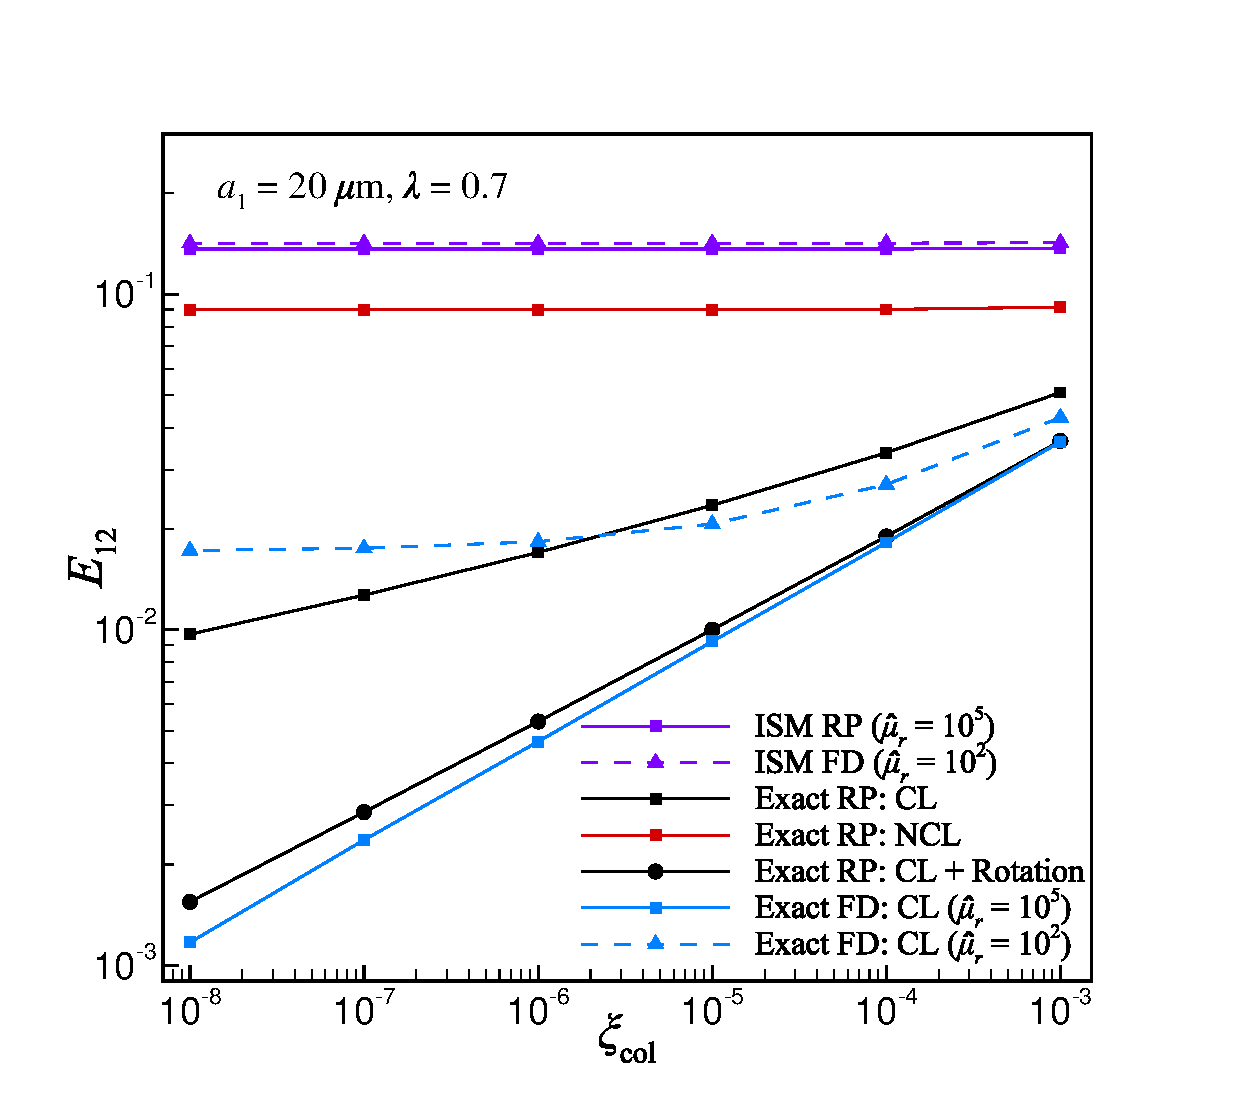
\includegraphics[trim=05mm 05mm 25mm 20mm, clip, width=0.6\textwidth]{../figs/PRF/fig9.pdf}
\caption{Collision efficiency evaluated using different collision gaps}
\label{fig:cut}
\end{figure}%%%%%%%%%%%%%%%%%%%%%%%%%%%%%%%%%%%%%%%%%%
Finally, we examine the effect of the collision gap size on $E_{12}$ under different representations of aerodynamic interactions. The aim is to check the possibility of collision using solely the models examined in this analysis, that is without additional treatments such as collision gap model or van der Waals forces even though they strongly dominate the interaction between droplets at such small gaps. Therefore, the collision gap has to approach zero and such simulations are numerically challenging, especially for small $\lambda$. In all simulations discussed above the collision gap size was fixed and equal to $\xi_\text{col}=10^{-3}$. This new set of simulations is performed for $10^{-8}\leq\xi_\text{col}\leq10^{-3}$. Note that to obtain numerical convergence for smaller $\xi_\text{col}$, it is necessary to reduce the integration time step. Since we use an adaptive Runge--Kutta scheme, the size of $\Delta t$ is not fixed but assessed dynamically by local error estimation.

Figure~\ref{fig:cut} shows the collision efficiency computed using the collision gap model at different $\xi_\text{col}$. To reduce the computational cost, all simulations have been performed for the same setting of a larger droplet radius $a_1 = 20~\mu$m and $\lambda=0.7$. Each curve represents a different model of aerodynamic interactions. As expected, the simulations employing the approximate ISM representations are almost insensitive to $\xi_\text{col}$. Similarly, a rigid pair under non-continuum lubrication description yields a non-zero $E_{12}$ thanks to a slow logarithmically increasing resistance. For the other four cases $E_{12}$ decreases with $\xi_\text{col}$ which is the effect of the singularity in the resistance coefficients of approaching pairs under a continuum description. Consequently, for rigid particles with and without rotation (black lines) as well as fluid drops with a high viscosity ratio (solid blue line), $E_{12} \to 0$ as we shrink $\xi_\text{col}$. The exception here is a fluid pair with $\hat{\mu}_r=10^2$, showing that the decrease in $E_{12}$ levels out as $\xi_\text{col}$ is reduced. This is a result of resistance being proportional to $\xi^{-1/2}$ at a moderate $\hat{\mu}_r$, as opposed to $\xi^{-1}$ for the other three cases. Accordingly, for this force representation $E_{12}$ can be quantified without making use of the collision gap model or van der Waals forces. Such values are computed and presented in the Tables \ref{tab:E10}, \ref{tab:E20}, and \ref{tab:E30} of Appendix \ref{sec:E12}.


\subsection{Numerical performance}
Now we focus on numerical aspects of conducted simulations, including techniques, developments, tools, observations, issues, and challenges.
The motivation for this analysis is to check the applicability of different representations of aerodynamic interactions to perform complex simulations of the dynamics of many particles in turbulent flows.

\subsubsection{Computation time}
In terms of computational costs, the ISM features of relatively low complexity. Therefore, the results from the ISM are the fastest (seconds, in terms of wall-clock time) to obtain. At each time step the forces acting on the pair of droplets are computed by solving a small system of six equations that include three components of disturbance velocities at the location of each droplet. Computation time is much longer when employing exact representations of aerodynamic interactions, e.g.\ \cite{JO84}, and the solutions in bispherical coordinates for rigid \citep{SJ26,ONM70} or liquid \citep{HHS73,Z80} particles (minutes to hours). Rotation increases the computational cost (potentially by orders of magnitude depending on the problem) owing to the need for a much greater number of operations to calculate the forces, torques, coupling terms, and integrating two additional equations for the conservation of angular momentum, i.e.\ Equation~(\ref{eq:eqm3}).

The convergence rate of computing the interaction forces using the solutions in bispherical coordinates or the multipole expansion of \cite{JO84} slows down as the gap between droplets decreases. It should be noted, however, that the second approach is easier to implement in computer codes and offers better computational performance. This desired feature (a faster convergence) was obtained by combining analytical solutions for nearly touching spheres with infinite series that define resistance coefficients for large separations. In all the simulations considered here, we found that the multipole expansion provides satisfactory accuracy even when summing the first 100 terms. To achieve similar precision by using the solutions in bispherical coordinates we need to sum up about $10^3$ terms. Another factor influencing computational time is the particle radius ratio. For smaller $\lambda$, the calculation of aerodynamic interactions takes a longer time as more terms must be added up, so that the summations reach their limits. This applies in particular to the resistances given by \cite{ONM70} for the motion of unequal particles in a direction perpendicular to their line of centers. Therefore, the smaller the radius ratio or spacing between the particles, the larger the system of equations to be solved. Moreover, for pairs with substantially different sizes the systems can be ill-conditioned. Another impact of the radius ratio on computation time comes from the differences in the settling speed. As $\lambda \to 1$, the pair approaches at a much slower relative velocity since $\Delta W \to 0$, so the first RHS component in Figure~\ref{fig:decomp} diminishes. In this limit, the equations of motion must be integrated for longer periods of time to allow the particles to collide.

Apart from the aspects discussed above, the computation time is significantly influenced by the integration scheme. To solve the equations of motion, Equations~(\ref{eq:eqm1})--(\ref{eq:eqm3}), three different schemes were employed: (i) fourth-order Adams--Bashforth, (ii) classical fourth-order Runge--Kutta, and (iii) adaptive Runge--Kutta that dynamically adjusts $\Delta t$ based on error estimations. All these schemes led to the same results. As expected, the best performance was achieved with the adaptive Runge--Kutta.

\subsubsection{Algorithm parallelization}

In a study by \cite{RWMG11}, the initial condition $y_0$, i.e.\ the off-center horizontal separation, was successively modified (in subsequent generations) by making use of the standard bisection method. The entire range of collision efficiency $E_{12} \in [0, 1]$ was scanned until further divisions of the sub-range did not show any significant change in $E_{12}$. Regrettably, such an approach features of a fairly low convergence rate.

\begin{figure}%fig:scal_fig:scal_fig:scal_fig:scal
\center
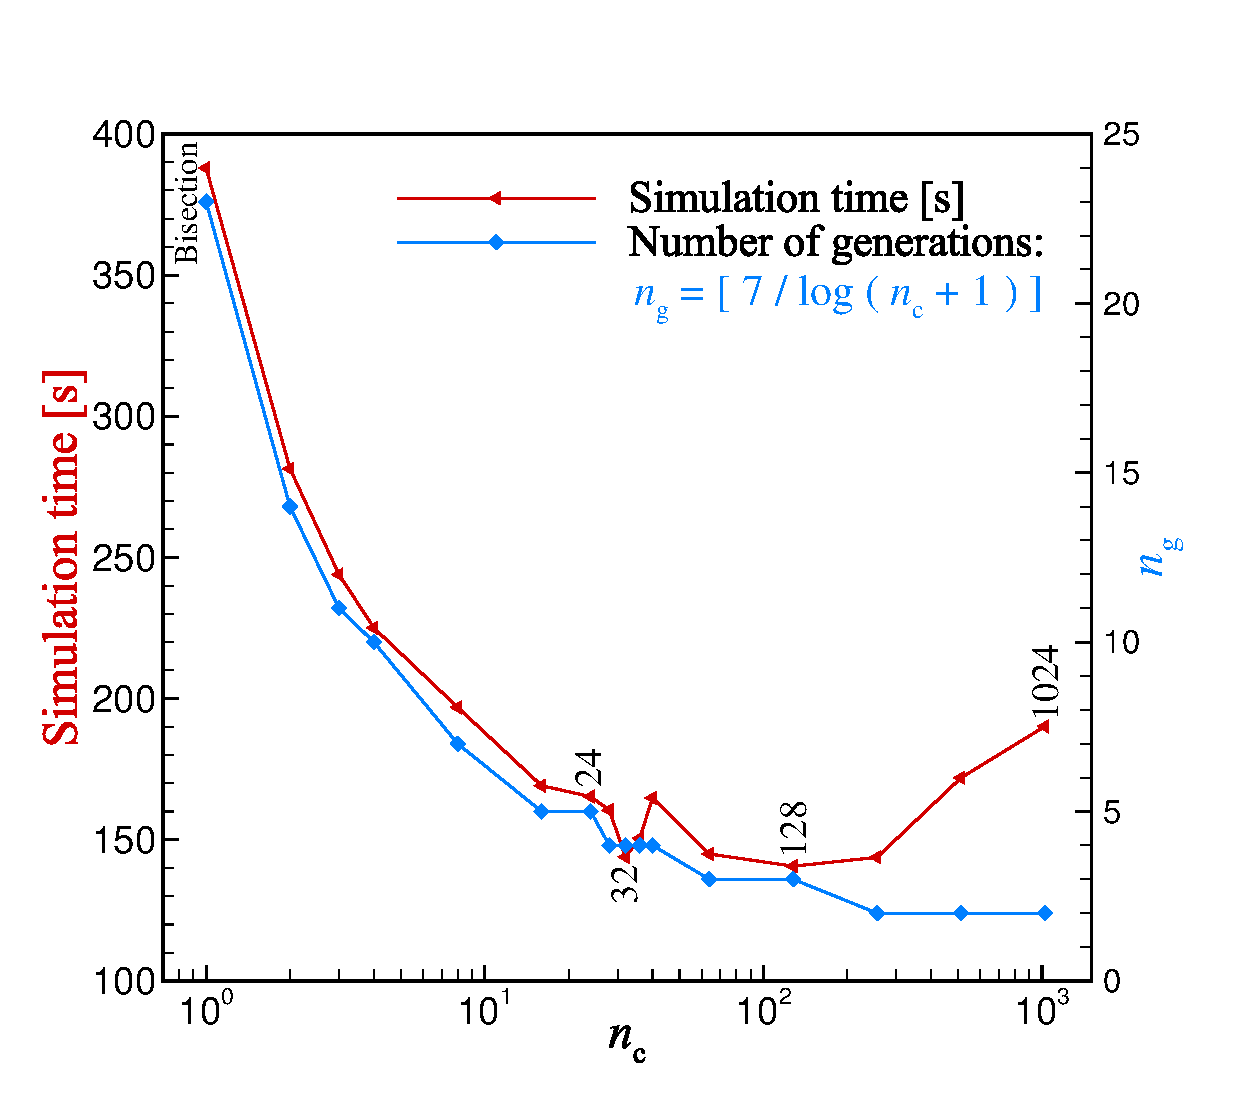
\includegraphics[trim=05mm 00mm 05mm 20mm, clip, width=0.6\textwidth]{../figs/PRF/fig10.pdf}
\caption{Change in simulation time and number of generations with the number of processes in $\log_{10}$ scale}
\label{fig:scal}
\end{figure}%%%%%%%%%%%%%%%%%%%%%%%%%%%%%%%%%%%%%%

A relatively simple remedy to speed up the computation is to parallelize the algorithm via MPI (Message Passing Interface library). For this purpose, we adopt the idea that is based on the multi-threaded bisection search. In the serial approach, the considered range that defines the collision efficiency is halved in subsequent generations, while in the parallel code the range of interest is divided by $n_\text{c} + 1$ where $n_\text{c}$ is the number of processes (sub-generations performed with different initial aims) each given to a computational core. Computations in subsequent generations are carried out with the same number of processors but for a much narrower starting range than in the serial method. This significantly reduces the number of generations needed to obtain accurate results.

In Figure~\ref{fig:scal} the left vertical axis refers to the change in the total simulation time (the wall clock time) for a set of twenty simulations carried out with different number of processors, shown in $\log_{10}$ scale, assuming $a_1=10~\mu$m and $\lambda=0.05$ to $0.99$. The right vertical axis shows number of generations ($n_\text{g}$) required to narrow down the initial range $[0,1]$ to the desired accuracy of $10^{-7}$ in $E_{12}$. These measured quantities are plotted as a function of the number of processes. To achieve the accuracy, in subsequent $n_\text{g}$ generations, the considered (narrowing) range was divided into $n_\text{c} + 1$ sub-ranges in such a way that
\begin{eqnarray}
\frac{1}{(n_\text{c}+1)^{n_\text{g}}}\leq 10^{-7}. \nonumber
\label{eq:ng}
\end{eqnarray}

Figure~\ref{fig:scal} demonstrates that both lines follow a similar monotonic trend up to $n_\text{c}=128$. The reason for the decline in performance for $n_\text{c}>128$ is that all sub-generations (processes) start simultaneously but do not finish at the same time. Note that each subsequent generation begins when all the processes of the previous generation are completed. Consequently, there is a certain idle time as the completed processes must wait for those that are still in progress. For a large $n_\text{c}$, there is a significant difference in simulation time between the fastest and slowest processes. This difference negatively impacts computing performance, especially in the early generations. On the other hand, the favorable performance obtained for $n_\text{c}\leq128$ is a consequence of the higher scanning resolution. Since the machine we were using has 24-core processors, most of the simulations in were performed using $n_\text{c}=24$.

%%%%%   E N D   R E S U L T S   %%%%%

\subsection{Summary}%%%%%   C O N C L U S I O N S   %%%
This aim of current discussion was to quantify the collision efficiency of two non-deformably spherical particles settling under gravity in quiescent air. The investigations were carried out by means of numerical simulations employing our in-house code. Most of the simulations were performed using settings characteristic for typical cloud droplets. An accurate description of this process finds an important application in numerical weather prediction systems. To test sensitivity of the numerical model, additional simulations at different relative viscosities were also performed. A number of cases were considered assuming different sizes and radius ratios of the particle pairs. The main focus, however, was on small droplets with radii in the range 0.5 to 30~$\mu$m.

The governing equation for particle motion includes various representations of the aerodynamic interaction. This is the main element of novelty and important extension of previous studies on this topic. The interacting forces and torques were evaluated using both an approximate method and exact solutions to the Stokes equation for two spheres. Other important effects analyzed here are related to the non-continuum lubrication and internal circulation of the water inside droplets. The obtained results are compared with reference data available in the literature. The comparison shows that the collision efficiency computed using the approximate model (ISM) or the non-continuum lubrication is usually larger than that of rigid particles moving in a continuous medium. In the considered range of parameters, the increase in $E_{12}$ for the non-continuum lubrication varies from $25$ to $125$\%. As for the liquid particles, the collision efficiency is also enhanced compared to the rigid pair. This enhancement may reach even $45$\%. The reason for this increase resides in a somewhat lower drag acting on the settling spheres. In the case of liquid particles, the drag force is partially mitigated by the mobile interface. In general, non-continuum lubrication has a larger impact on the collision efficiency compared to the internal circulation of drops which loses its influence as their inertia (size) increases. In numerical simulations, therefore, treating medium-sized cloud droplets as rigid particles is a reasonable assumption, but considering non-continuum effects in their aerodynamic interaction is expected to change the results. Further on, it has been demonstrated that the collision efficiency of liquid particles with a very large viscosity ratio is the same as that of freely rotating rigid spheres of the same density. 

The second part of this analysis deals with the numerical aspects. Computing the aerodynamic interactions comes with a huge computational cost. The numerical complexity is particularly problematic when using solutions in bispherical coordinates. It should be noted that these interactions have to be calculated at every time step for different separation distances and radius ratios. To speed up the computation, the code was parallelized using the MPI libraries. In this way, we were able to obtain results in a much shorter time and with greater accuracy.

This study is a step forward to model multi-particle systems in turbulent flows. Therefore, one potentially significant direction of future research is to implement different representations of aerodynamic interactions in a code for hybrid DNS. This paves the way for a more realistic modeling of cloud processes.

%%%%%   E N D   C O N C L U S I O N S   %%%%%
%\subsection{Data Availability}%%%%%%%%%%%%%%%%%%%%%%%%%%%%%%%%%%%%%%%
\paragraph{Data Availability\label{sec:data}}
The code for computing hydrodynamic interaction is available in \url{https://github.com/aababaei/Two-Sphere-Interaction}. It was developed both to plot the figures in this subsection and calculate forces and torques in the equations of motion. The resistance functions were taken from the research web-page of David Jeffrey: \url{https://www.uwo.ca/apmaths/faculty/jeffrey/research/Resistance.html}.


%\bibliographystyle{bibstyle}
%\bibliography{references}
\newpage
\end{document}
